\documentclass[14pt,letterpaper,hidelinks]{extarticle}
%\usepackage[ansinew]{inputenc}
\usepackage[utf8x]{inputenc}
%\usepackage[latin1]{inputenc}
\usepackage[spanish]{babel}
\usepackage[letterpaper,includeheadfoot, top=1cm, bottom=3.0cm, right=2.0cm, left=2.0cm]{geometry}
\renewcommand{\familydefault}{\sfdefault}

\usepackage{svg}

\usepackage{graphicx}
\usepackage{color}
\usepackage{hyperref}
\usepackage{amssymb}
\usepackage{url}
%\usepackage{pdfpages}
\usepackage{fancyhdr}
\usepackage{hyperref}
\usepackage{subfig}
\usepackage{indentfirst}
\usepackage{titlesec}
\titleformat*{\section}{\large\bfseries}
\titleformat*{\subsection}{\normalsize\bfseries}

\usepackage{listings} %Codigo
\lstset{language=C, tabsize=4,framexleftmargin=5mm,breaklines=true}

\begin{document}
\thispagestyle{empty}
\renewcommand*\listtablename{Índice de tablas}
\renewcommand{\contentsname}{\'Indice}
\renewcommand*{\refname}{}

%\begin{sf}
% --------------- ---------PORTADA --------------------------------------------
\newpage
\pagestyle{fancy}
\fancyhf{}
%-------------------- CABECERA ---------------------
\hbox{
\includegraphics[scale=0.3]{img/fcfm_dcc_png.png} }
%------------------ TÍTULO -----------------------
\vspace*{4cm}
\begin{center}
\Huge  {Tarea 1 - Búsqueda en Texto}\\
\vspace{1cm}
\Large {CC4102 - Diseño y Análisis de Algoritmos}\\
\end{center}

%----------------- NOMBRES ------------------------
\vfill
\begin{flushright}
\begin{table}[h]
	\large
  \raggedleft
	\begin{tabular}{ll}
		Alumnos&: Sebastián González\\
				&\ \ Patricio Isbej\\
		Profesor&: Gonzalo Navarro\\
		Auxiliar&: Jorge Bahamonde\\
		Fecha&: \today
	\end{tabular}
\end{table}
\end{flushright}

% ·············· ENCABEZADO - PIE DE PAGINA ············
\newpage
\pagestyle{fancy}
\fancyhf{}

%Encabezado
%\fancyhead[L]{\rightmark}
\fancyhead[L]{\small \rm \textit{Sección \nouppercase\rightmark}} %Izquierda
\fancyhead[R]{\small \rm \textbf{\thepage}} %Derecha


%\fancyfoot[L]{\small \rm \textit{Pie de página - Izquierda}} %Izquierda
%\fancyfoot[R]{\small \rm \textit{Pie de página - Derecha}} %Derecha
%\fancyfoot[C]{\thepage} %Centro

\renewcommand{\sectionmark}[1]{\markright{\thesection.\ #1}}
\renewcommand{\headrulewidth}{0.5pt}
%\renewcommand{\footrulewidth}{0.5pt}

% =============== INDICE ===============
%
%\tableofcontents
%\listoffigures
%\listoftables

% =============== SECCIONES Y SUBSECCIONES ===============
\begin{abstract}
   En este trabajo se analizó 3 algoritmos distintos de búsqueda en texto, implementandolos,
	 ejecutandolos para distintos casos y comparando estos resultados.
\end{abstract}
\section{Introducción}
	Los algoritmos de búsqueda en texto son fundamentales debido a sus variadas aplicaciones como búsquedas dentro de documentos,
	búsqueda de cadenas de ADN, etc. Para este trabajo se compararon los siguientes algoritmos:
	\begin{itemize}
			\item Fuerza Bruta
			\item Knuth-Morris-Pratt
			\item Boyer-Moore-Horspool
	\end{itemize}
	\paragraph{} Fuerza Bruta consiste en buscar de izquierda a derecha partiendo del primer caracter del texto y patrón, comparando caracter a
	caracter, si se encuentra una diferencia se vuelve a comparar comenzando con el caracter siguiente en el texto del que se comenzó, y si
	se recorrió todo el patrón entonces hay un calce.
	\paragraph{} Knuth-Morris-Pratt opera de manera similar a Fuerza Bruta, precalculando una tabla del tamaño del patrón a buscar donde
	cada elemento indica si en la posición donde se encuentra hay un sufijo que sea prefijo del patrón, para así al llegar
	a una diferencia se puede saber si hay tal sufijo y poder saltarse todos esos caracteres.
	\paragraph{} Boyer-Moore-Horspool precalcula una operación "siguiente" para cada caracter que indica la última ocurrencia en el patrón
	de ese caracter (sin considerar su último caracter). Una vez calculado comienza a comparar desde la derecha y si encuentra una diferencia,
	revisa que caracter se encontraba y avanza de acuerdo a la operación calculada (mientras más al principio se encuentre la última ocurrencia,
	más se va a avanzar en el texto).

	\paragraph{} Los algoritmos fueron ejecutados con los siguientes tipos de datos:
	\begin{itemize}
			\item Alfabeto Binario
			\item ADN real
			\item ADN sintético
			\item Lenguaje Natural, caso real
			\item Lenguaje Natural, caso sintético
	\end{itemize}

\section{Hipótesis}
	Asumiendo $n$ como el tamaño de los datos, $m$ como el tamaño del patrón y $c$ como el tamaño del alfabeto se
	Formularon las siguientes hipótesis.

	Para todos los algoritmos, el tener un $c$ mayor significa aumentar la probabilidad de fallar, lo que hace que se tenga que
	avanzar en el texto con mayor frecuencia y así tener que hacer menos comparaciones y tomar menos tiempo.
	\subsection{Fuerza Bruta}
		Para Fuerza Bruta, en el peor caso la diferencia se va a encontrar siempre al final de la búsqueda,
		teniendo que hacer entonces $nm$ comparaciones. Lo que significa que el tiempo y las comparaciones van a crecer
		proporcionales a $m$.

	\subsection{Knuth-Morris-Pratt}
		Este algoritmo depende de que se tengan muchas subcadenas que sean prefijo del patrón, lo que significa que va a ser mejor que
		el primer algoritmo, pero no por mucho.

	\subsection{Boyer-Moore-Horspool}
		Este algoritmo se va a comportar mejor que los 2 anteriores por la forma en que salta en el texto
		al encontrar diferencias (si el caracter no se encuentra o se encuentra muy al principio se salta $m$).
		Para un $c$ pequeño, este algoritmo no va a ser tanto mejor que los anteriores, pero a medida que crezca,
		va a mejorar significativamente.

\section{Diseño e implementación}

\newpage
\section{Experimentos y resultados}

	\subsection{Algoritmos}
		Se ejecutaron los algoritmos 1000 veces para cada dato y largo de patrón, obteniendose los siguientes resultados.

		\begin{figure}[ht!]
			\centering
			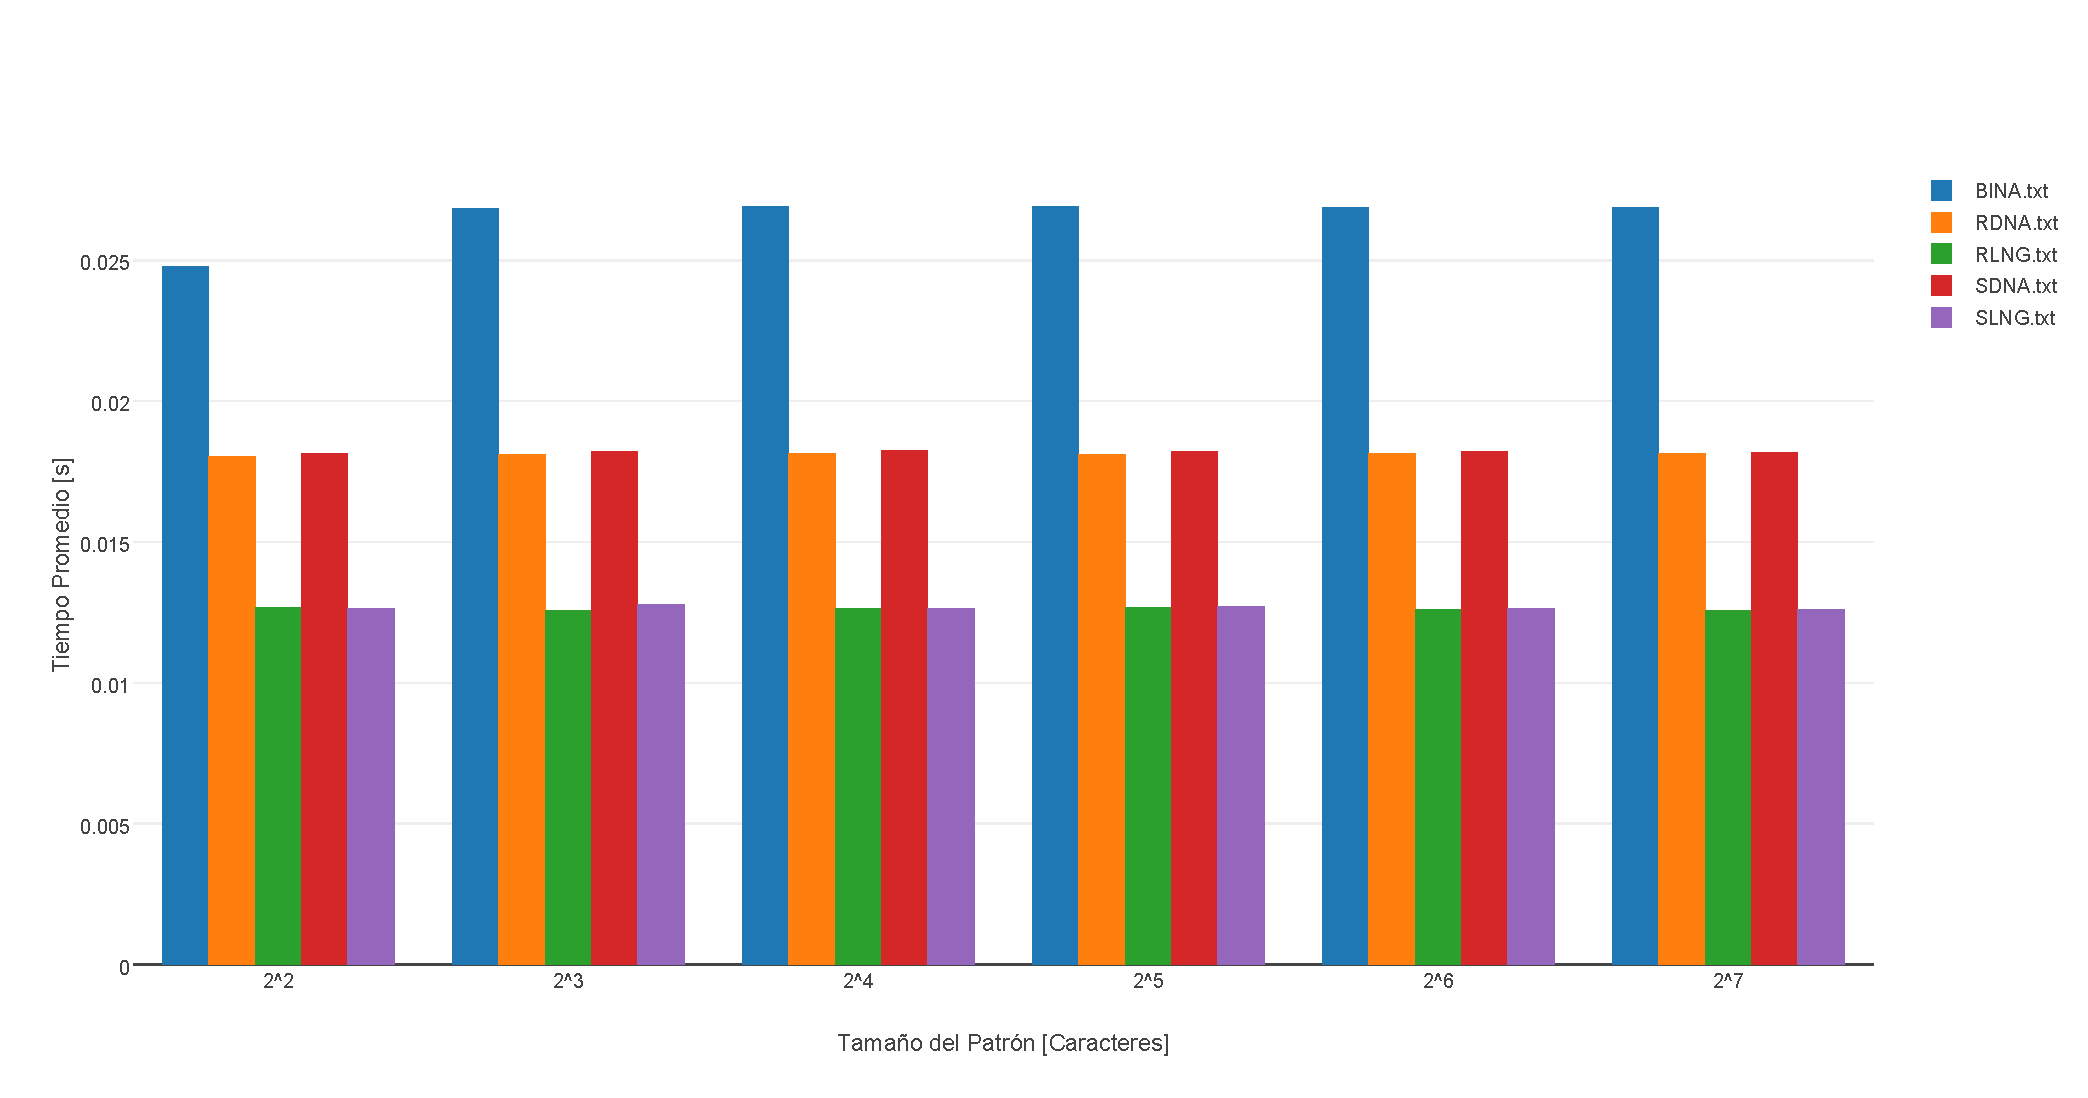
\includegraphics[scale=0.5]{img/tBF.pdf}
			\caption{Tiempo de promedio de búsqueda para Fuerza Bruta} \label{construccion}
		\end{figure}

	\newpage

		\begin{figure}[ht!]
			\centering
			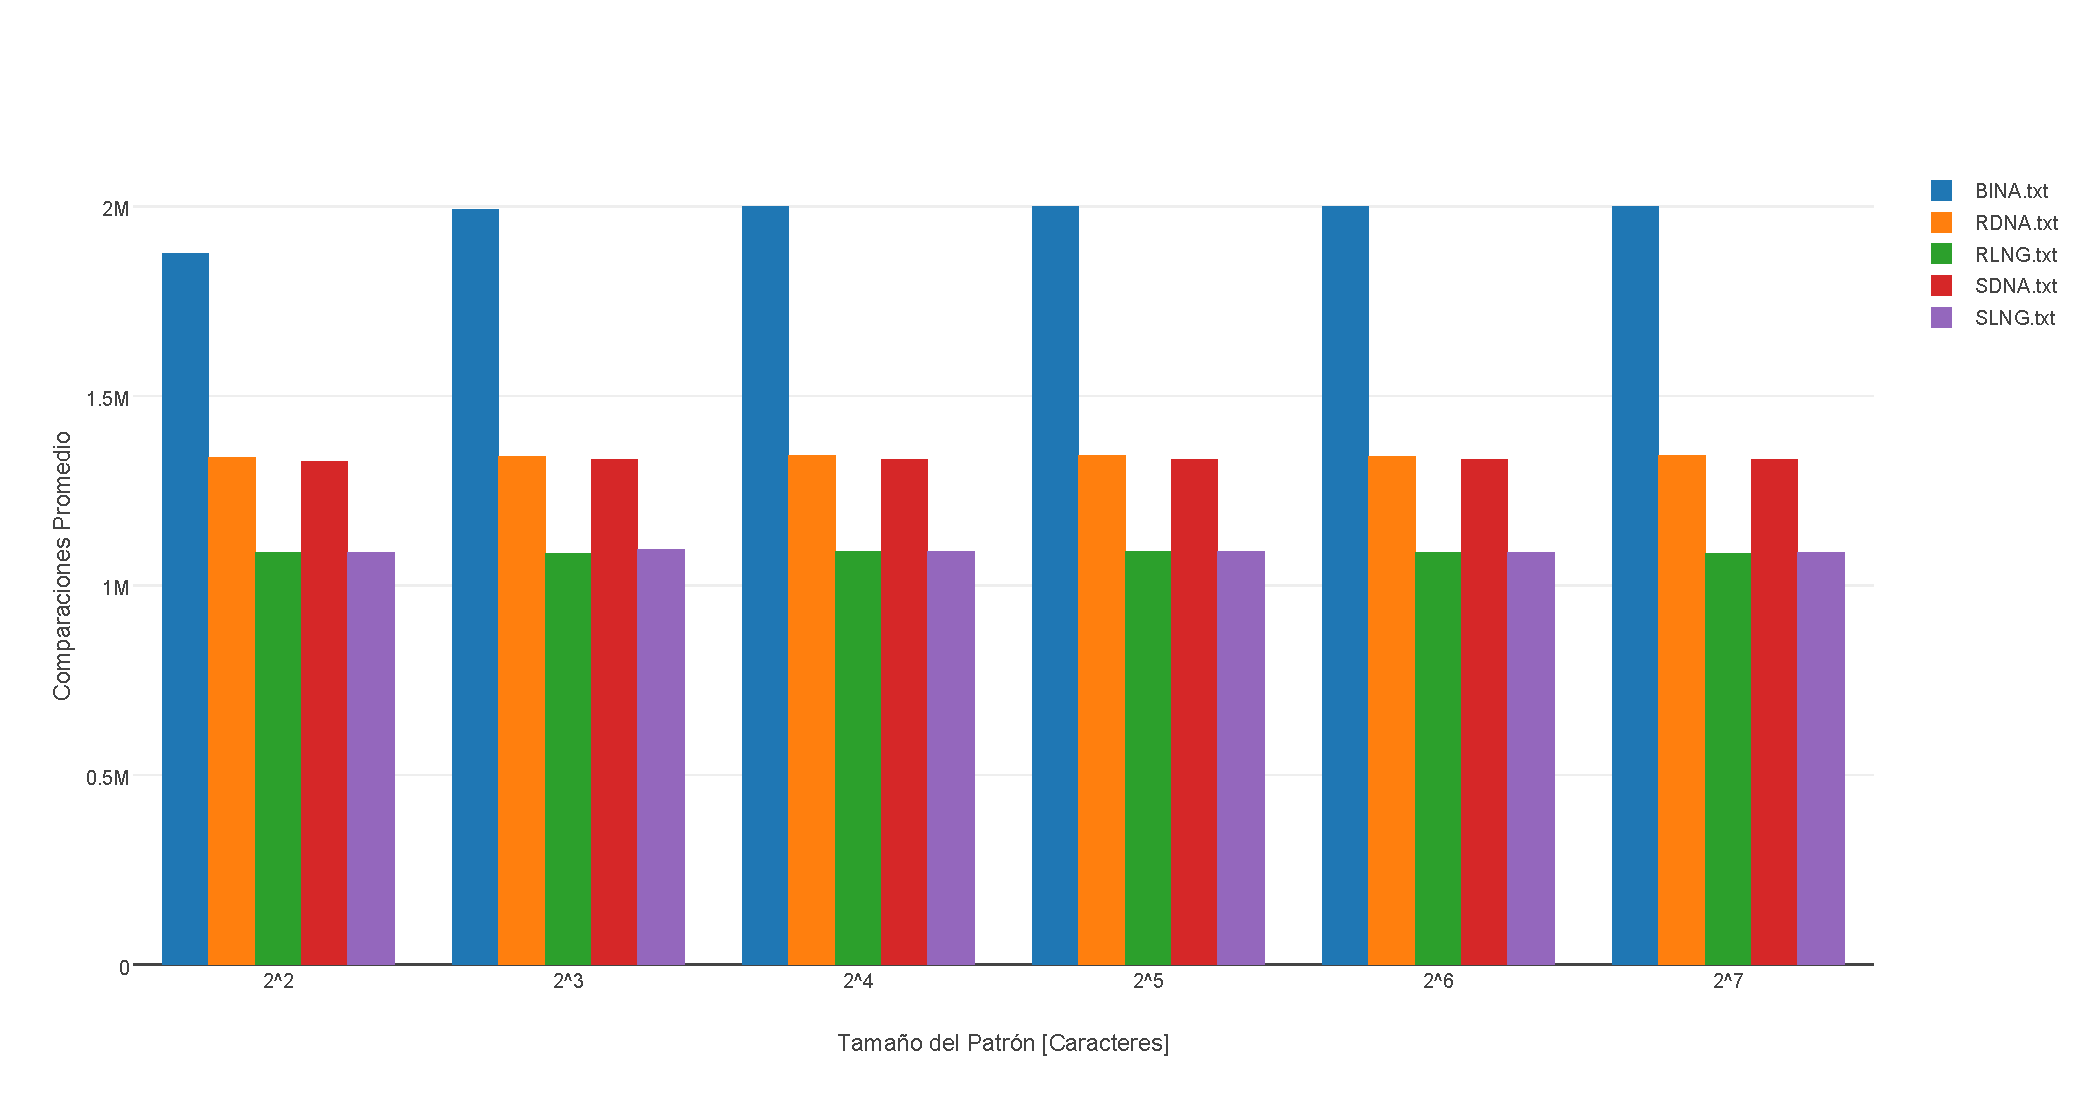
\includegraphics[scale=0.5]{img/cBF.pdf}
			\caption{Comparaciones promedio por búsqueda para Fuerza Bruta} \label{construccion}
		\end{figure}


		\begin{figure}[ht!]
			\centering
			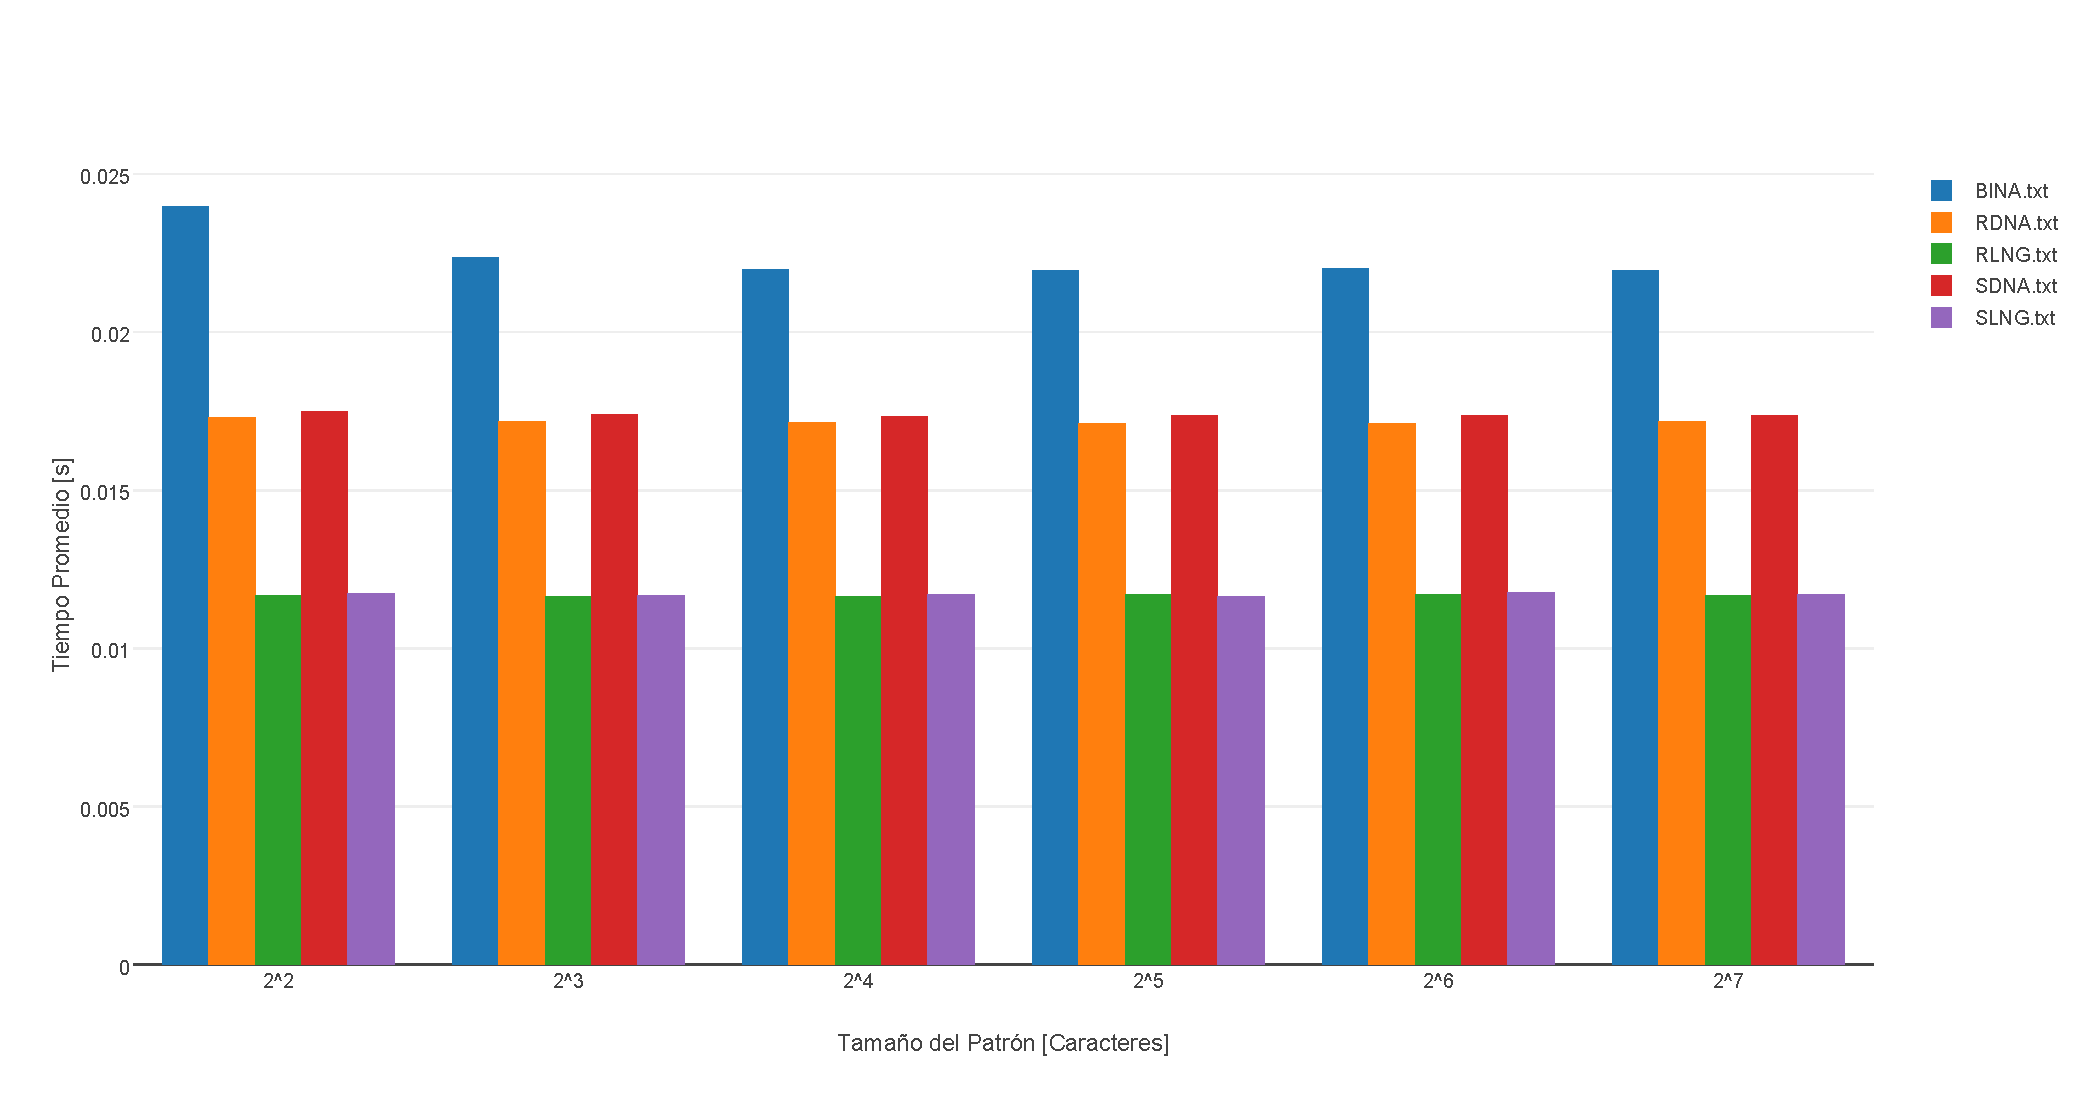
\includegraphics[scale=0.5]{img/tKMP.pdf}
			\caption{Tiempo de promedio de búsqueda para Knuth-Morris-Pratt} \label{construccion}
		\end{figure}

	\newpage
		\begin{figure}[ht!]
			\centering
			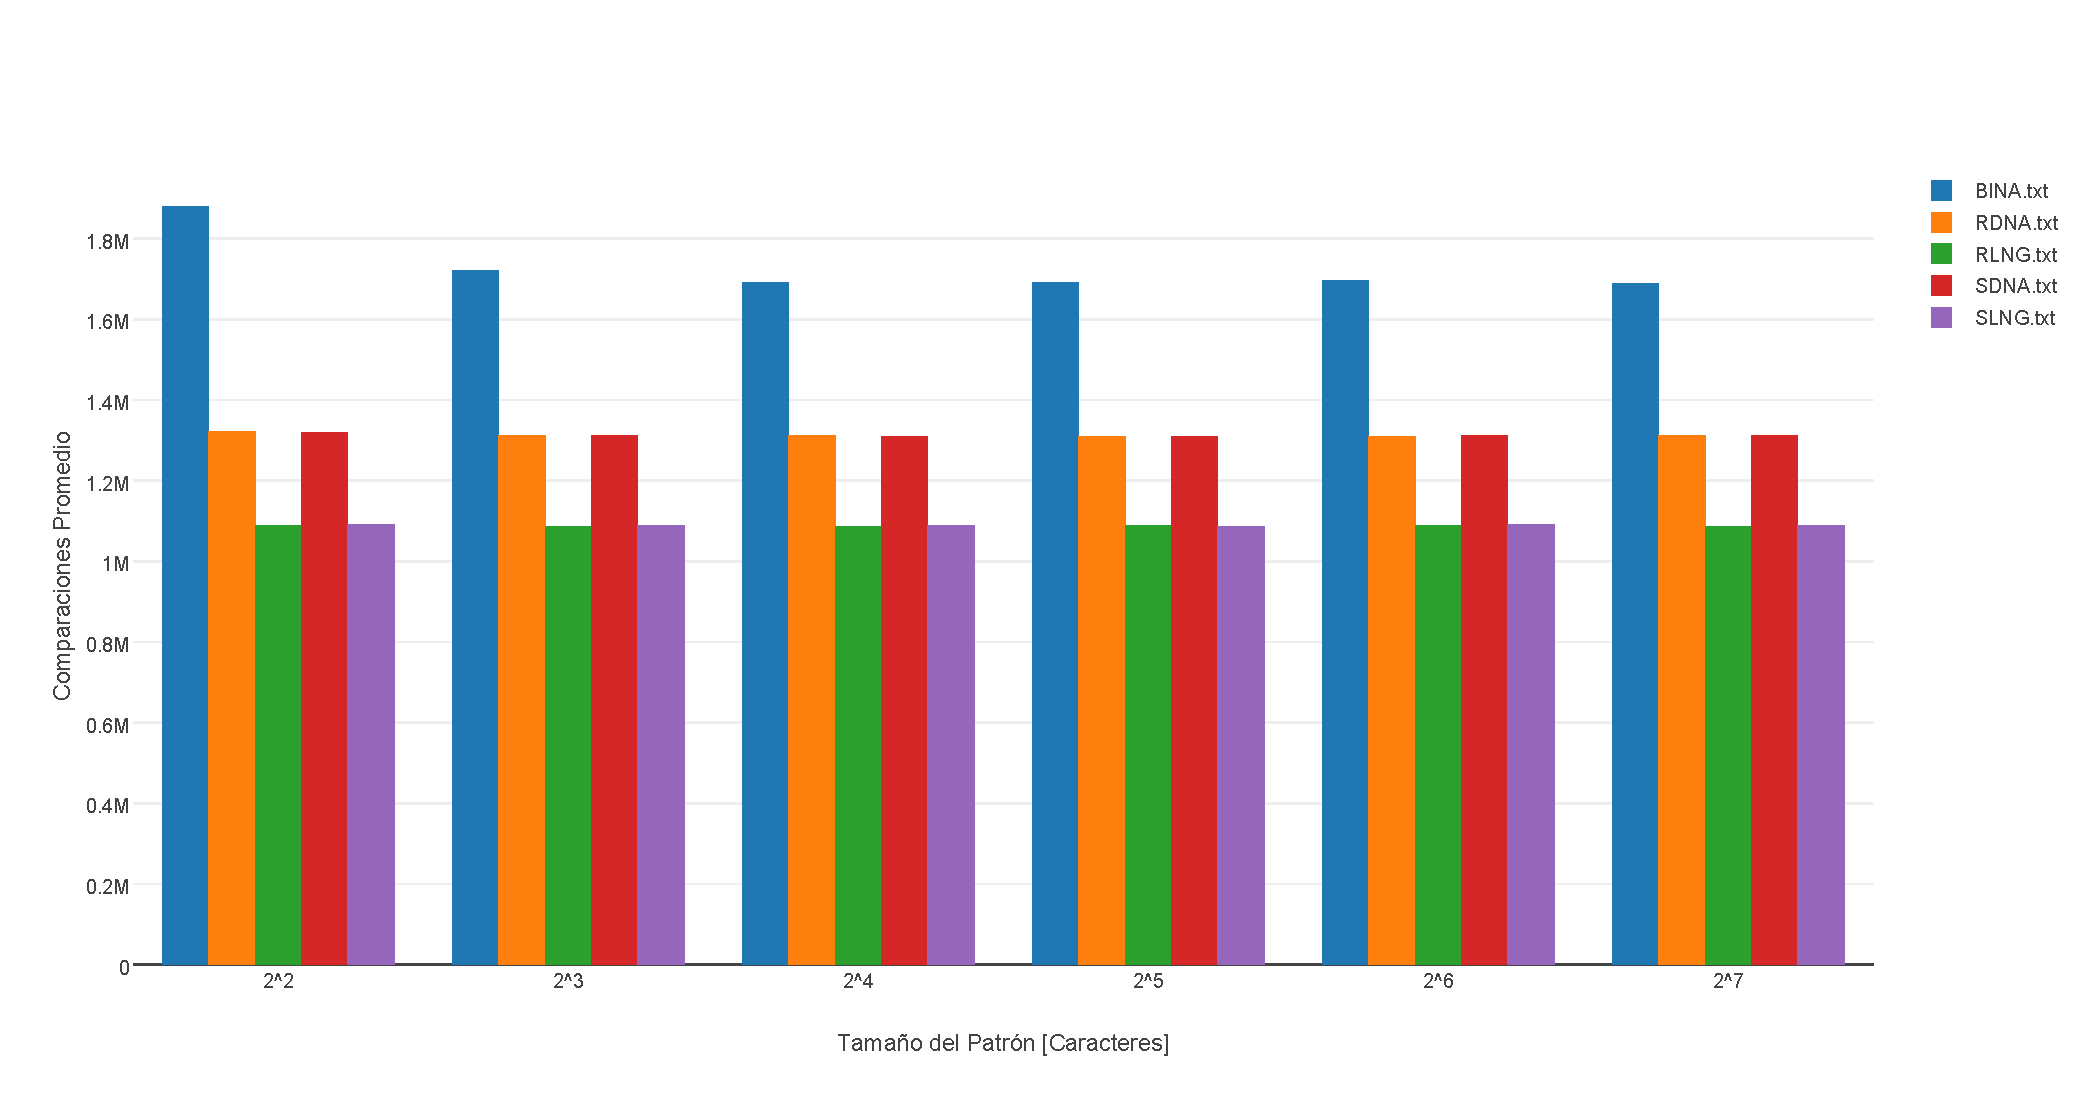
\includegraphics[scale=0.5]{img/cKMP.pdf}
			\caption{Comparaciones promedio por búsqueda para Knuth-Morris-Pratt} \label{construccion}
		\end{figure}


		\begin{figure}[ht!]
			\centering
			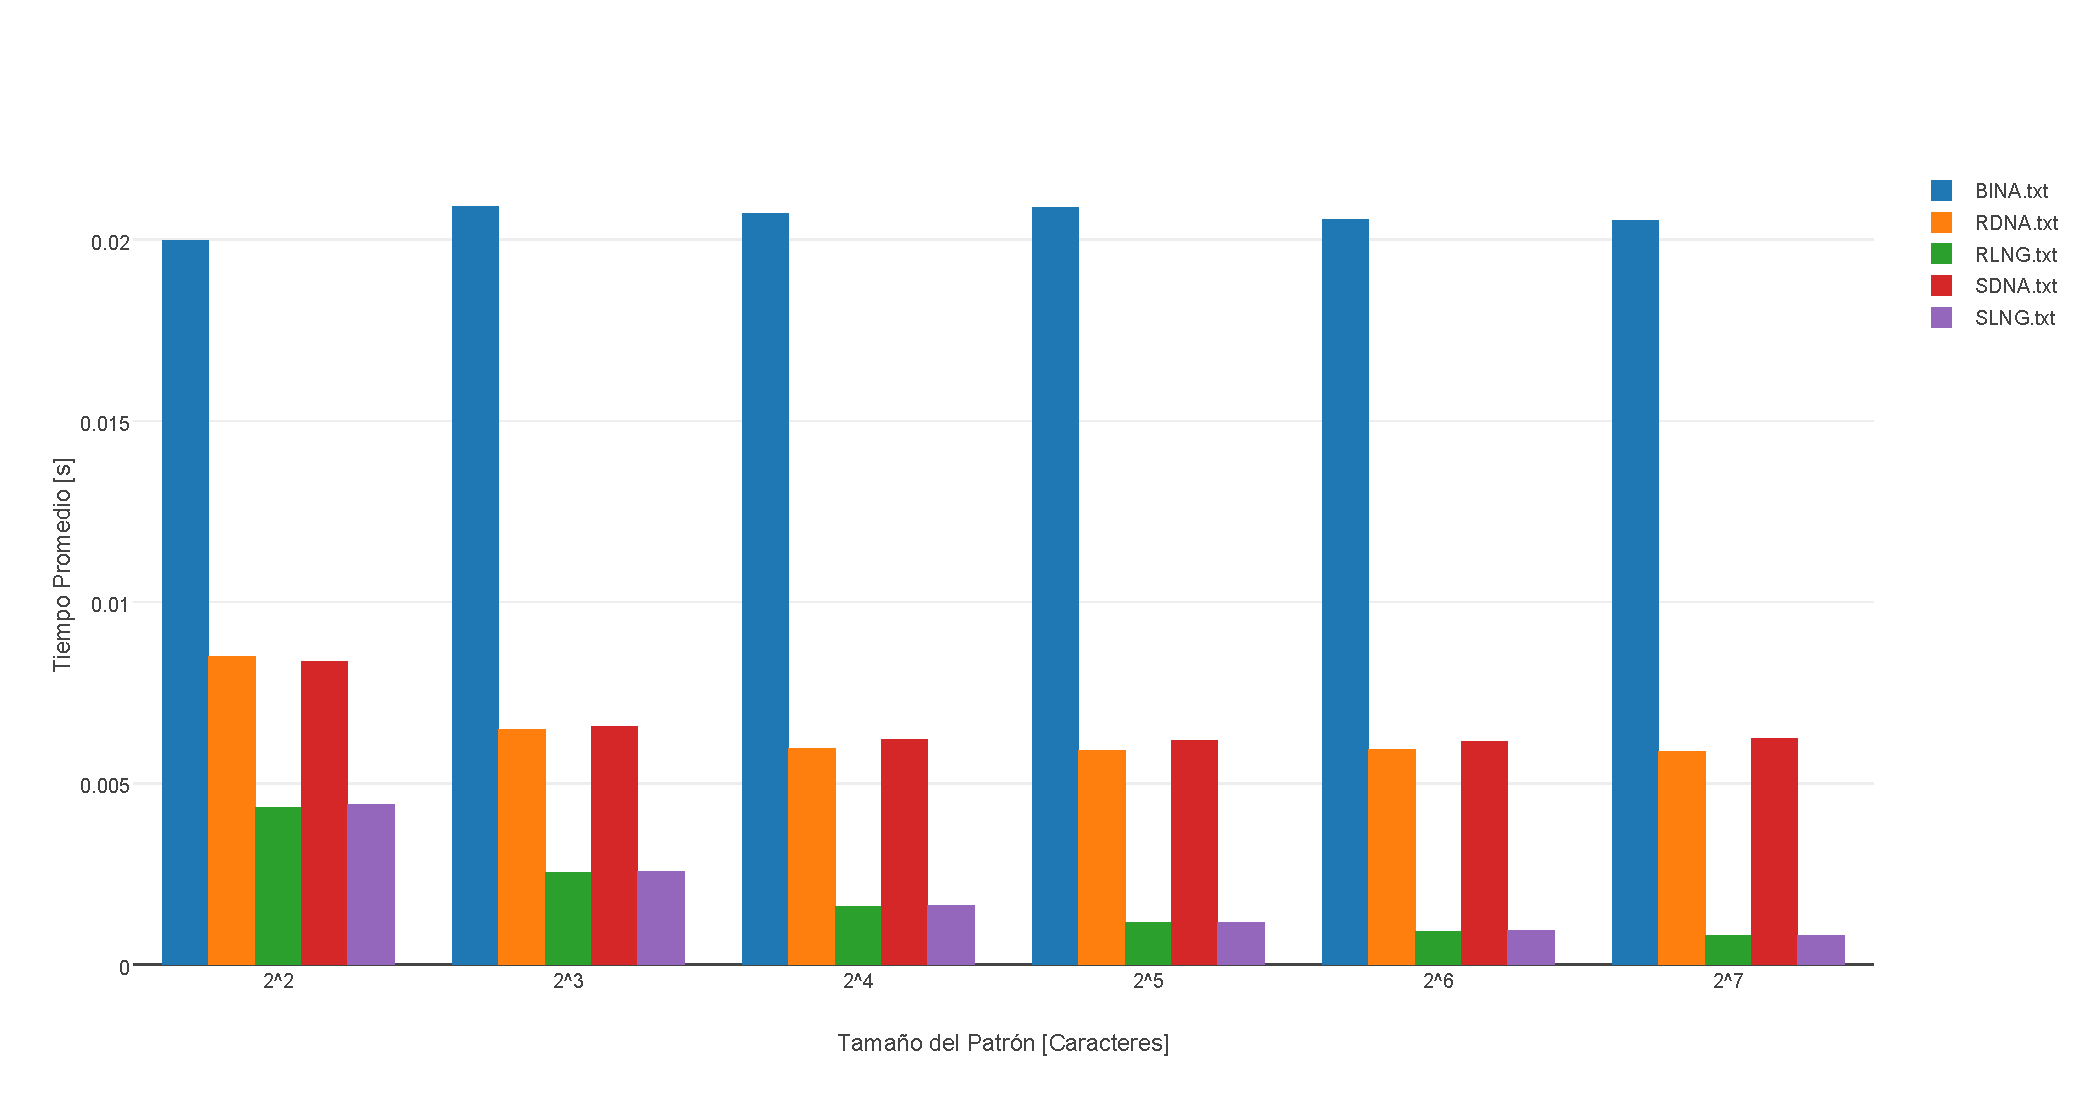
\includegraphics[scale=0.5]{img/tBMH.pdf}
			\caption{Tiempo de promedio de búsqueda para Boyer-Moore-Horspool} \label{construccion}
		\end{figure}

		\newpage
		\begin{figure}[ht!]
			\centering
			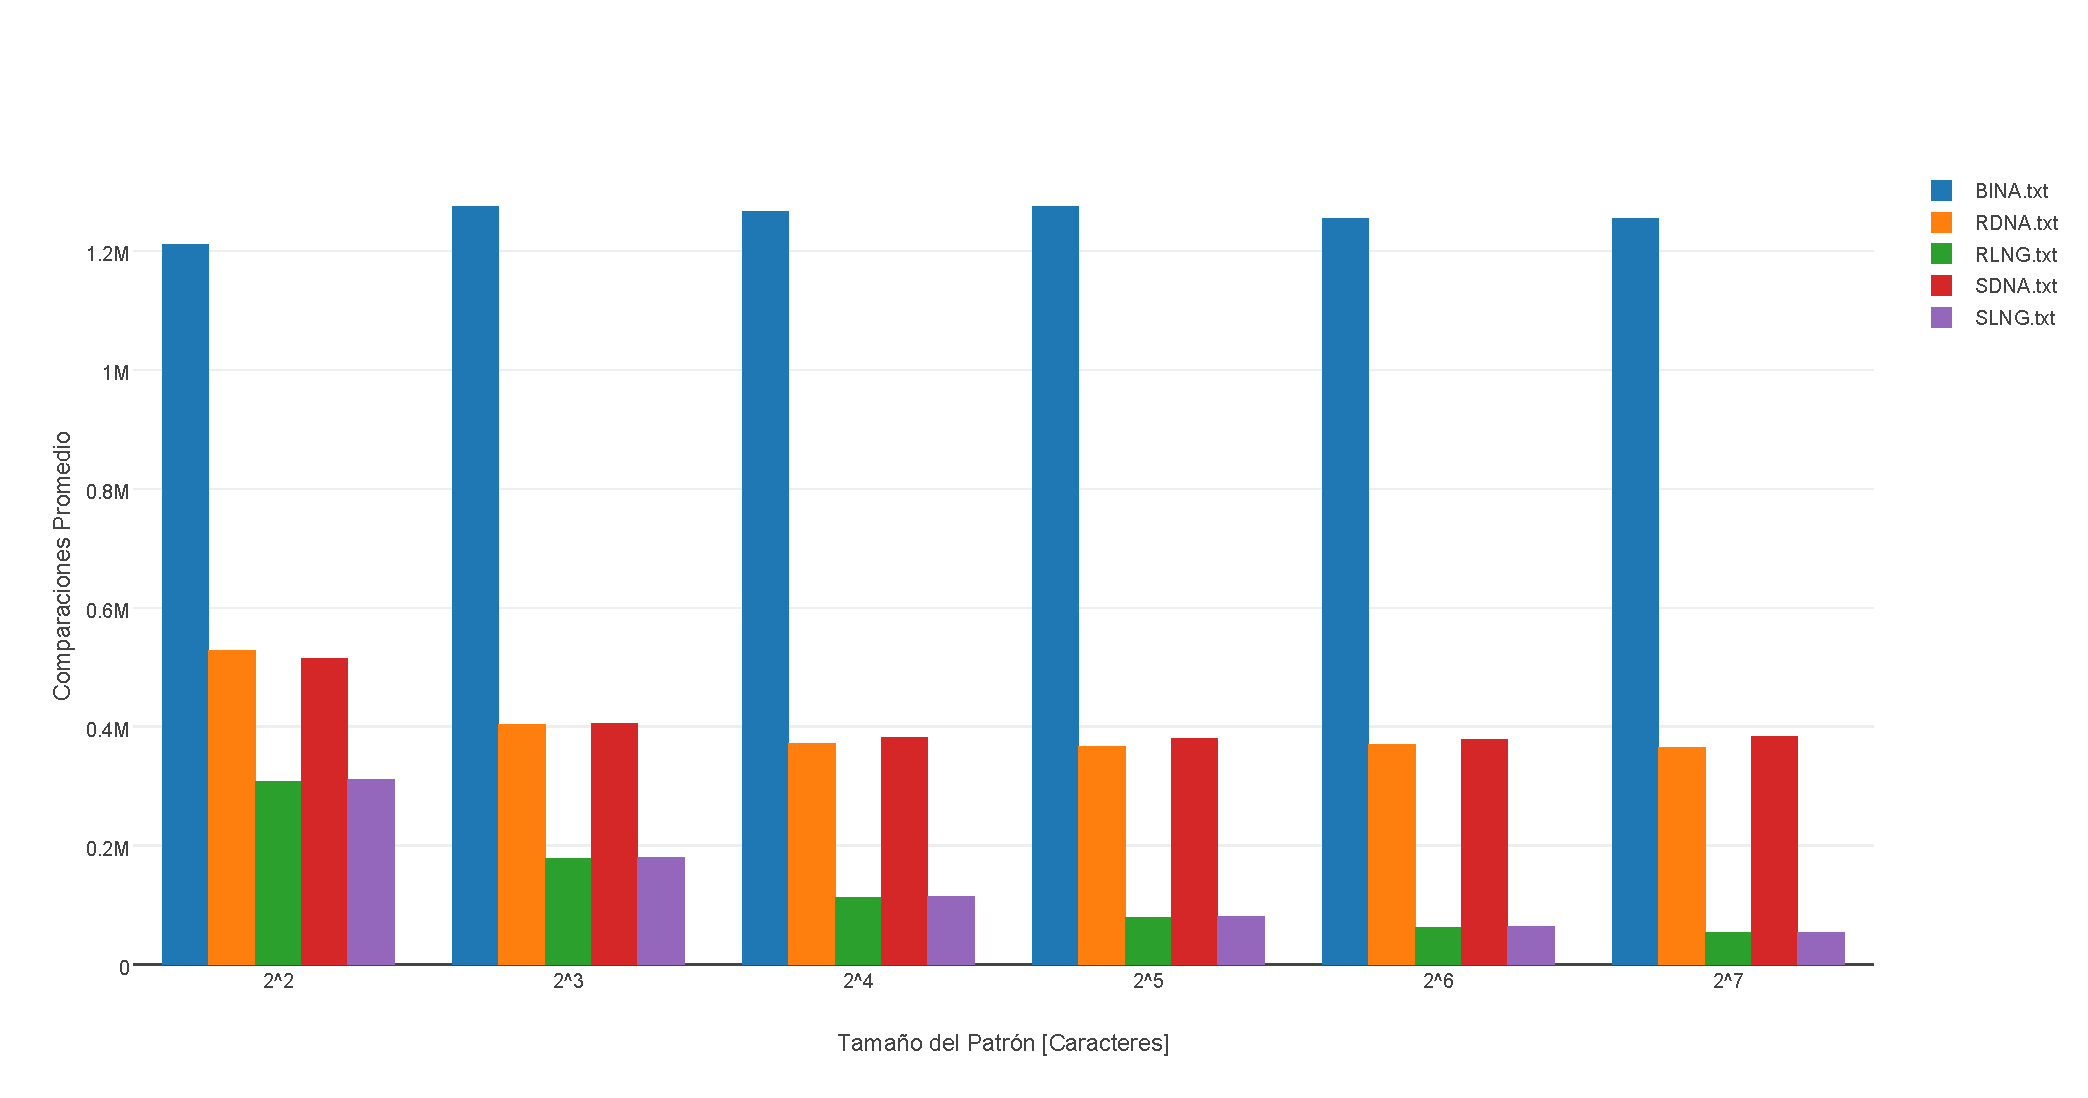
\includegraphics[scale=0.5]{img/cBMH.pdf}
			\caption{Comparaciones promedio por búsqueda para Boyer-Moore-Horspool} \label{construccion}
		\end{figure}


\newpage

	\subsection{Datos}
	Ordenando los resultados por datos (eliminando los casos sintéticos ya que resultaron similares a los naturales) se obtiene
		\begin{figure}[ht!]
			\centering
			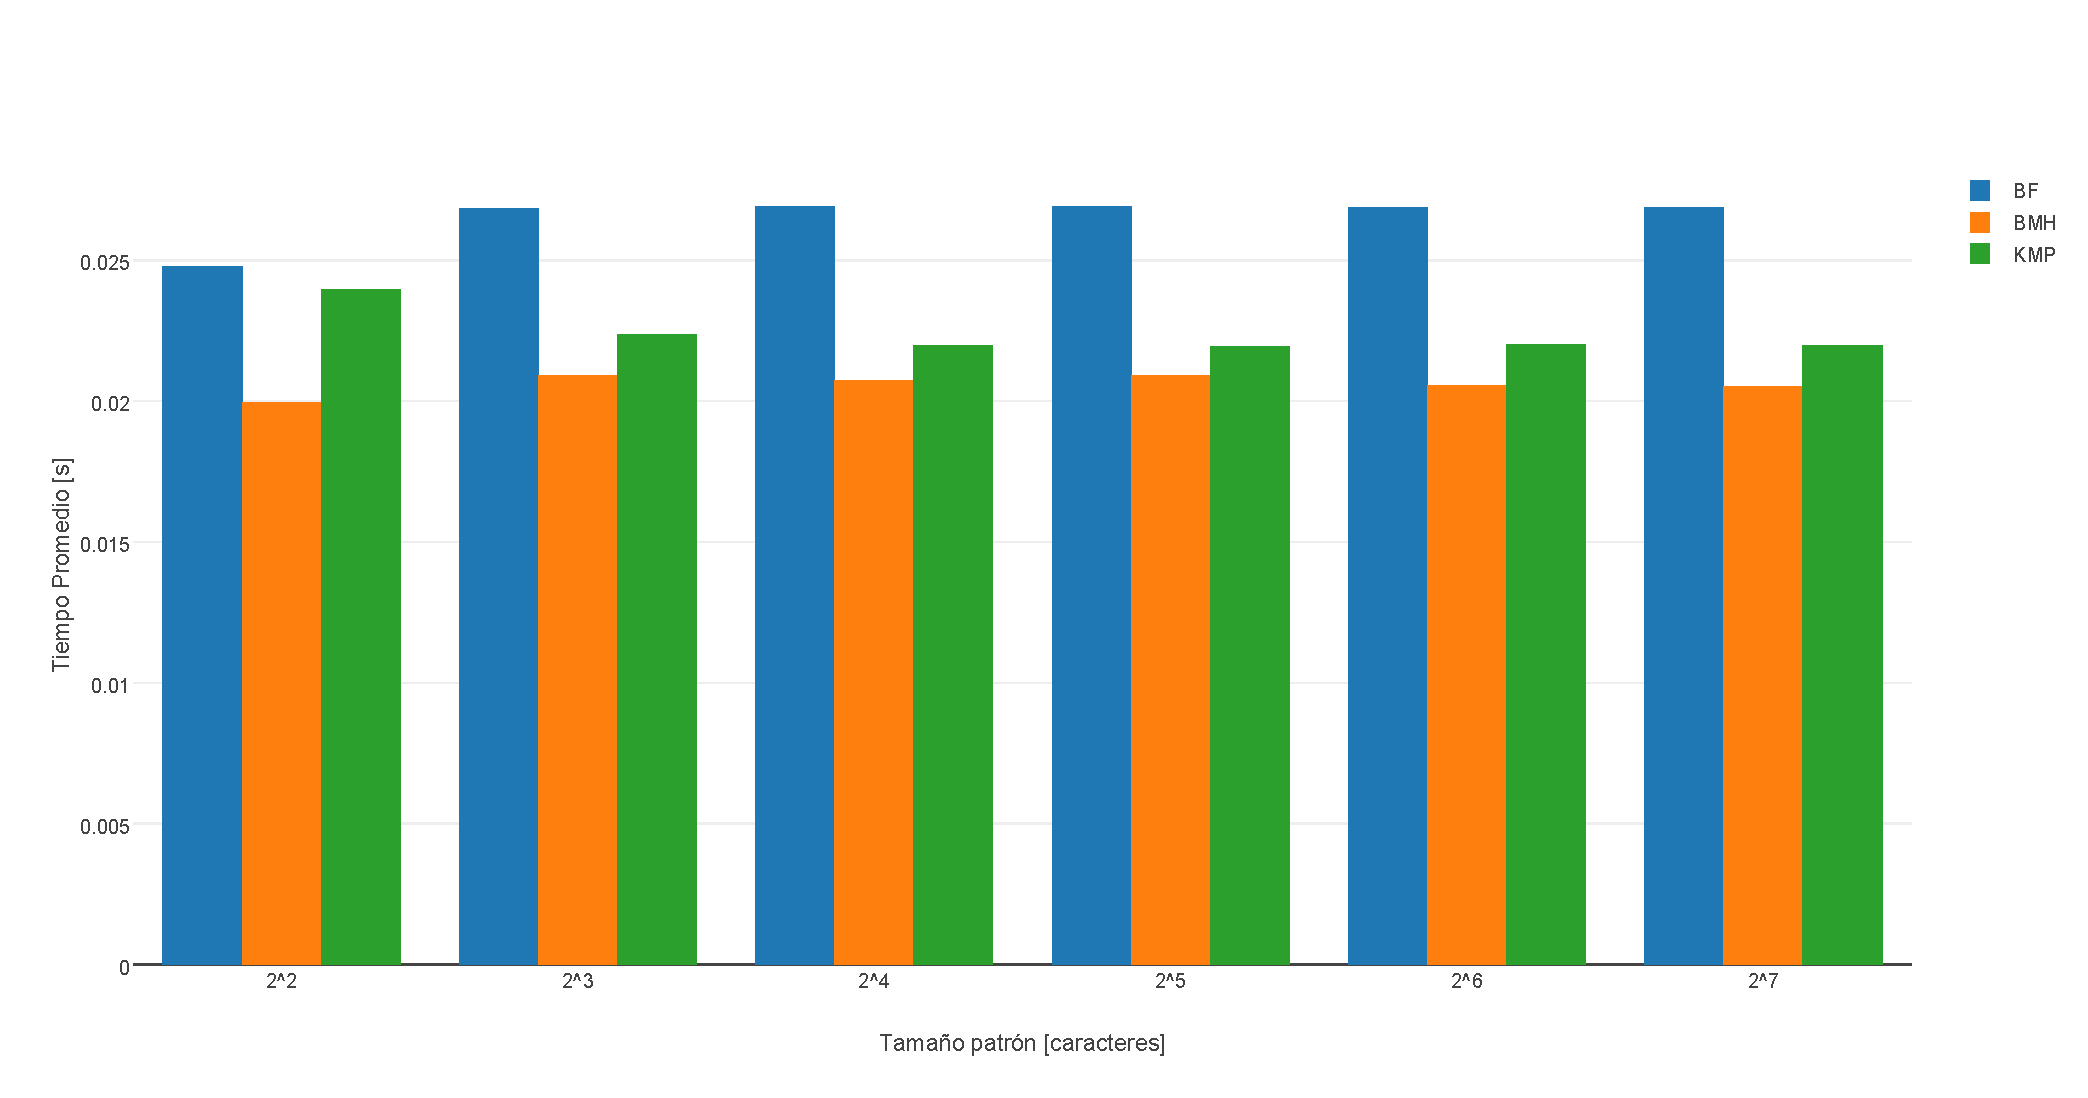
\includegraphics[scale=0.5]{img/tBINA.pdf}
			\caption{Tiempo promedio de búsqueda para texto binario} \label{construccion}
		\end{figure}
			\newpage
		\begin{figure}[ht!]
			\centering
			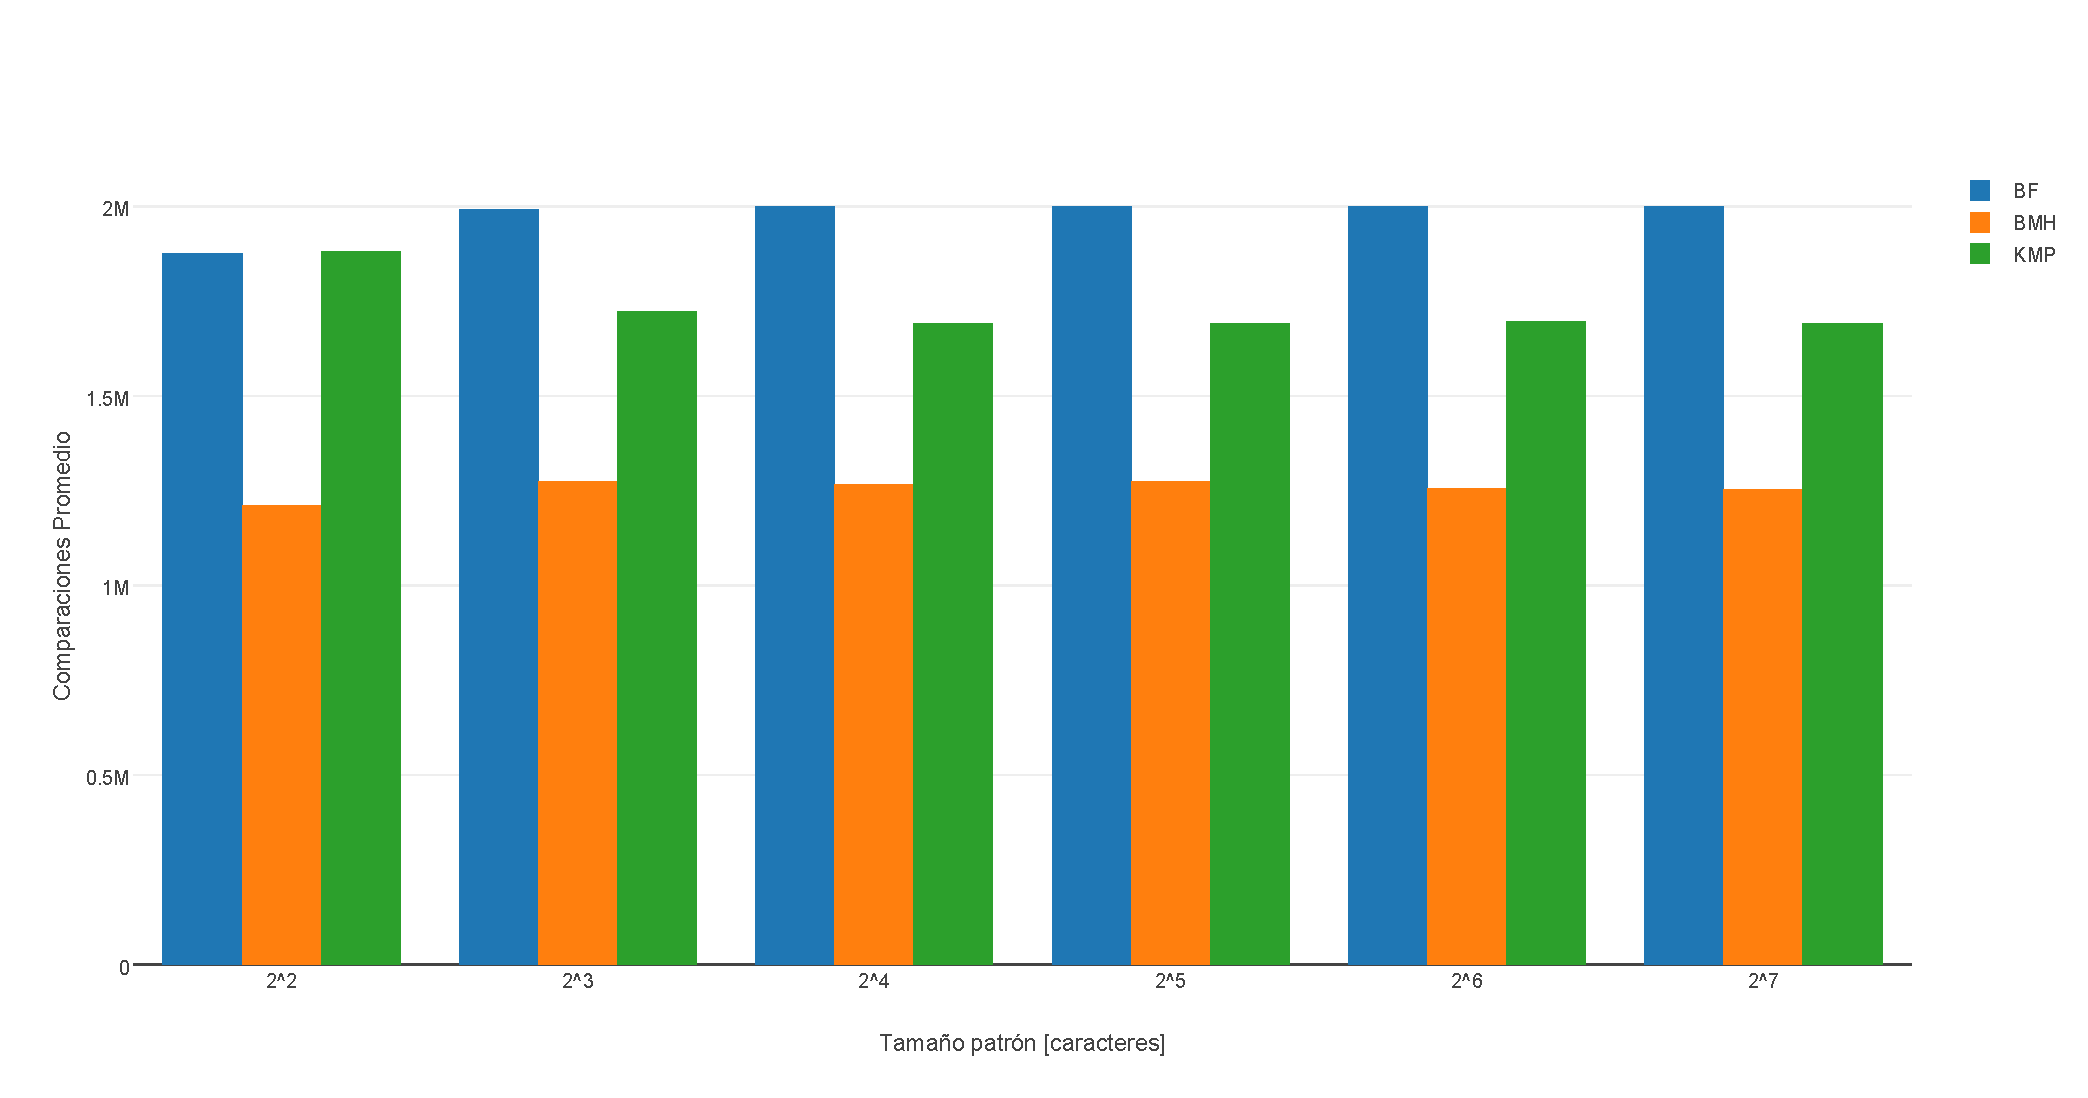
\includegraphics[scale=0.5]{img/cBINA.pdf}
			\caption{Comparaciones promedio por búsqueda para texto binario} \label{construccion}
		\end{figure}
	\newpage
		\begin{figure}[ht!]
			\centering
			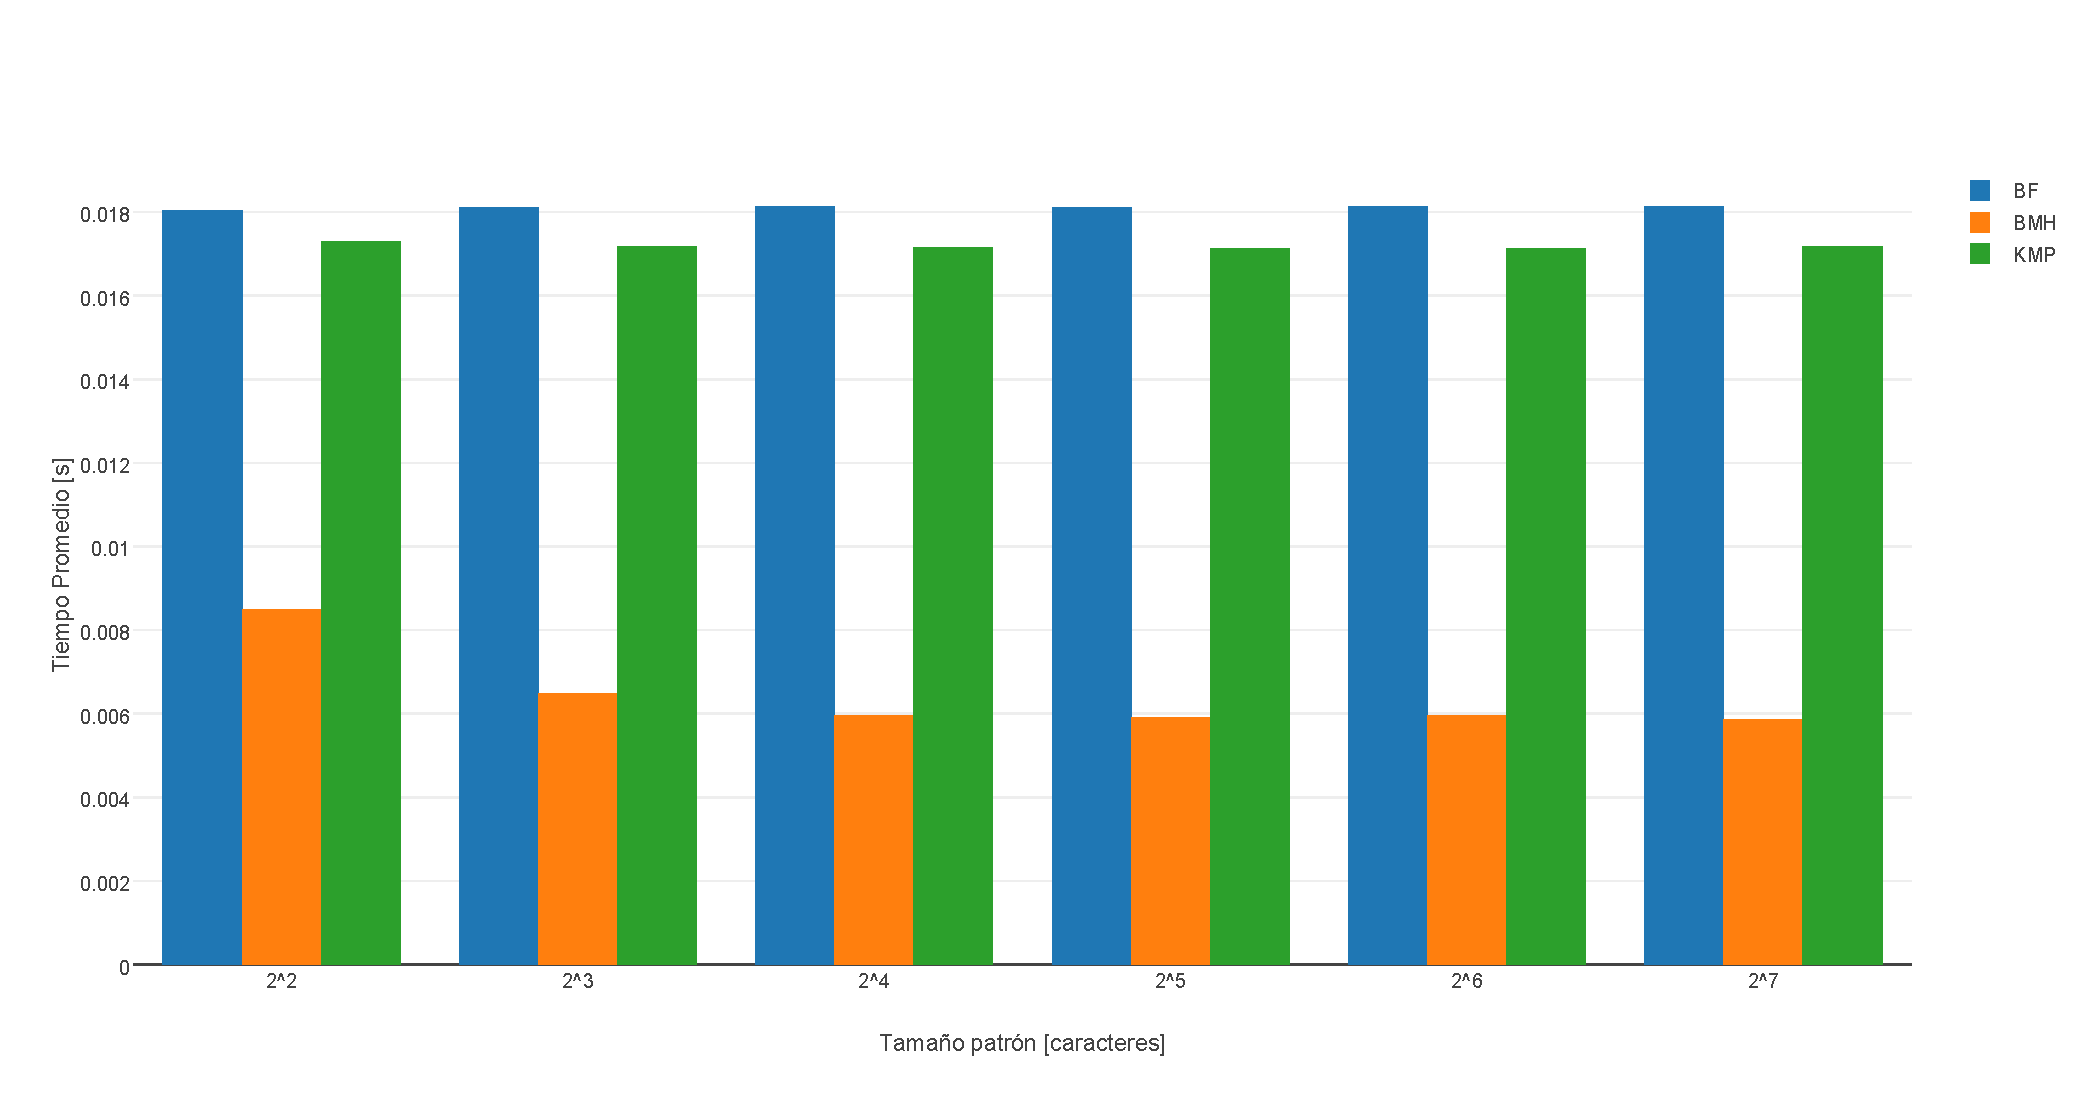
\includegraphics[scale=0.5]{img/tRDNA.pdf}
			\caption{Tiempo promedio de búsqueda para cadenas de ADN} \label{construccion}
		\end{figure}
			\newpage
		\begin{figure}[ht!]
			\centering
			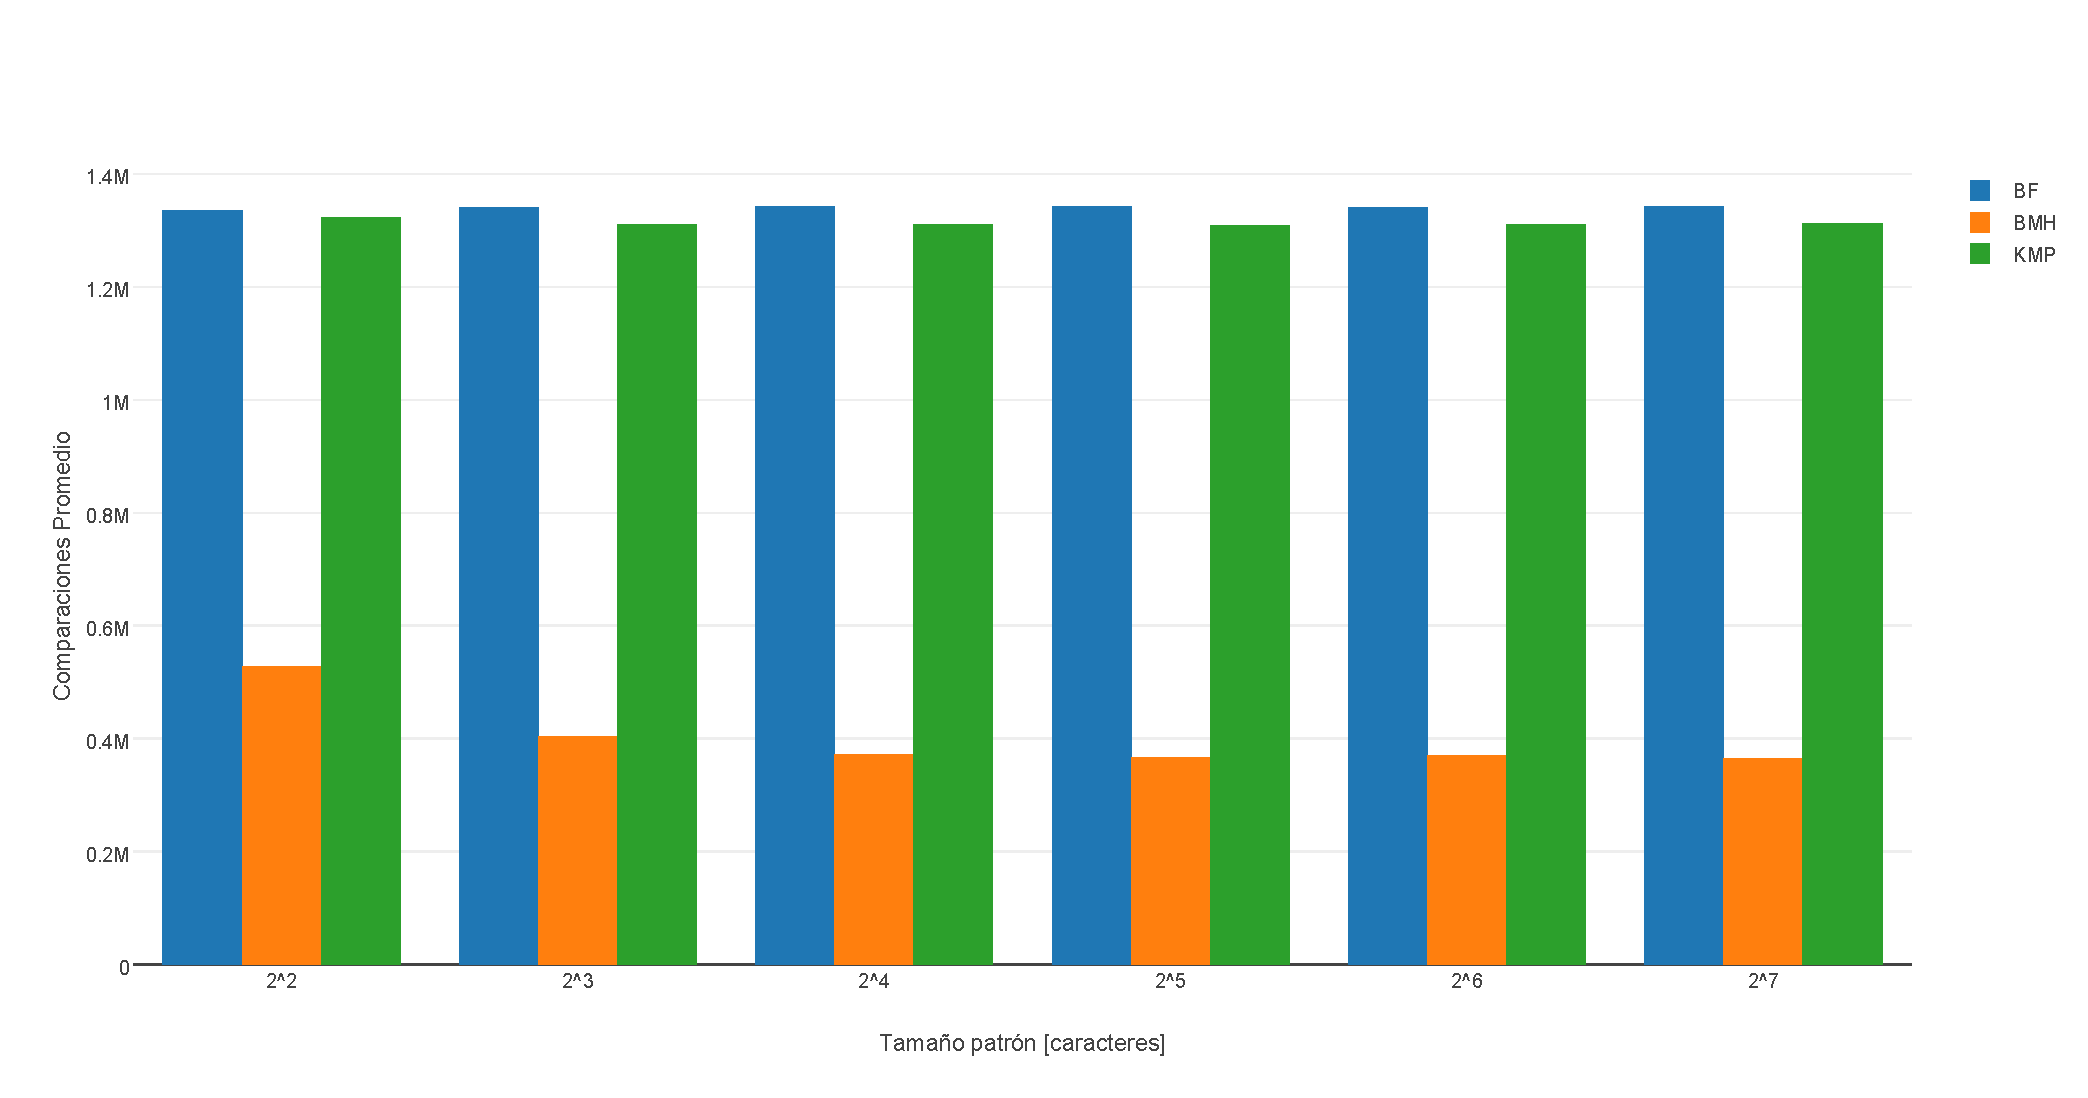
\includegraphics[scale=0.5]{img/cRDNA.pdf}
			\caption{Comparaciones promedio por búsqueda para cadenas de ADN} \label{construccion}
		\end{figure}

	\newpage
		\begin{figure}[ht!]
			\centering
			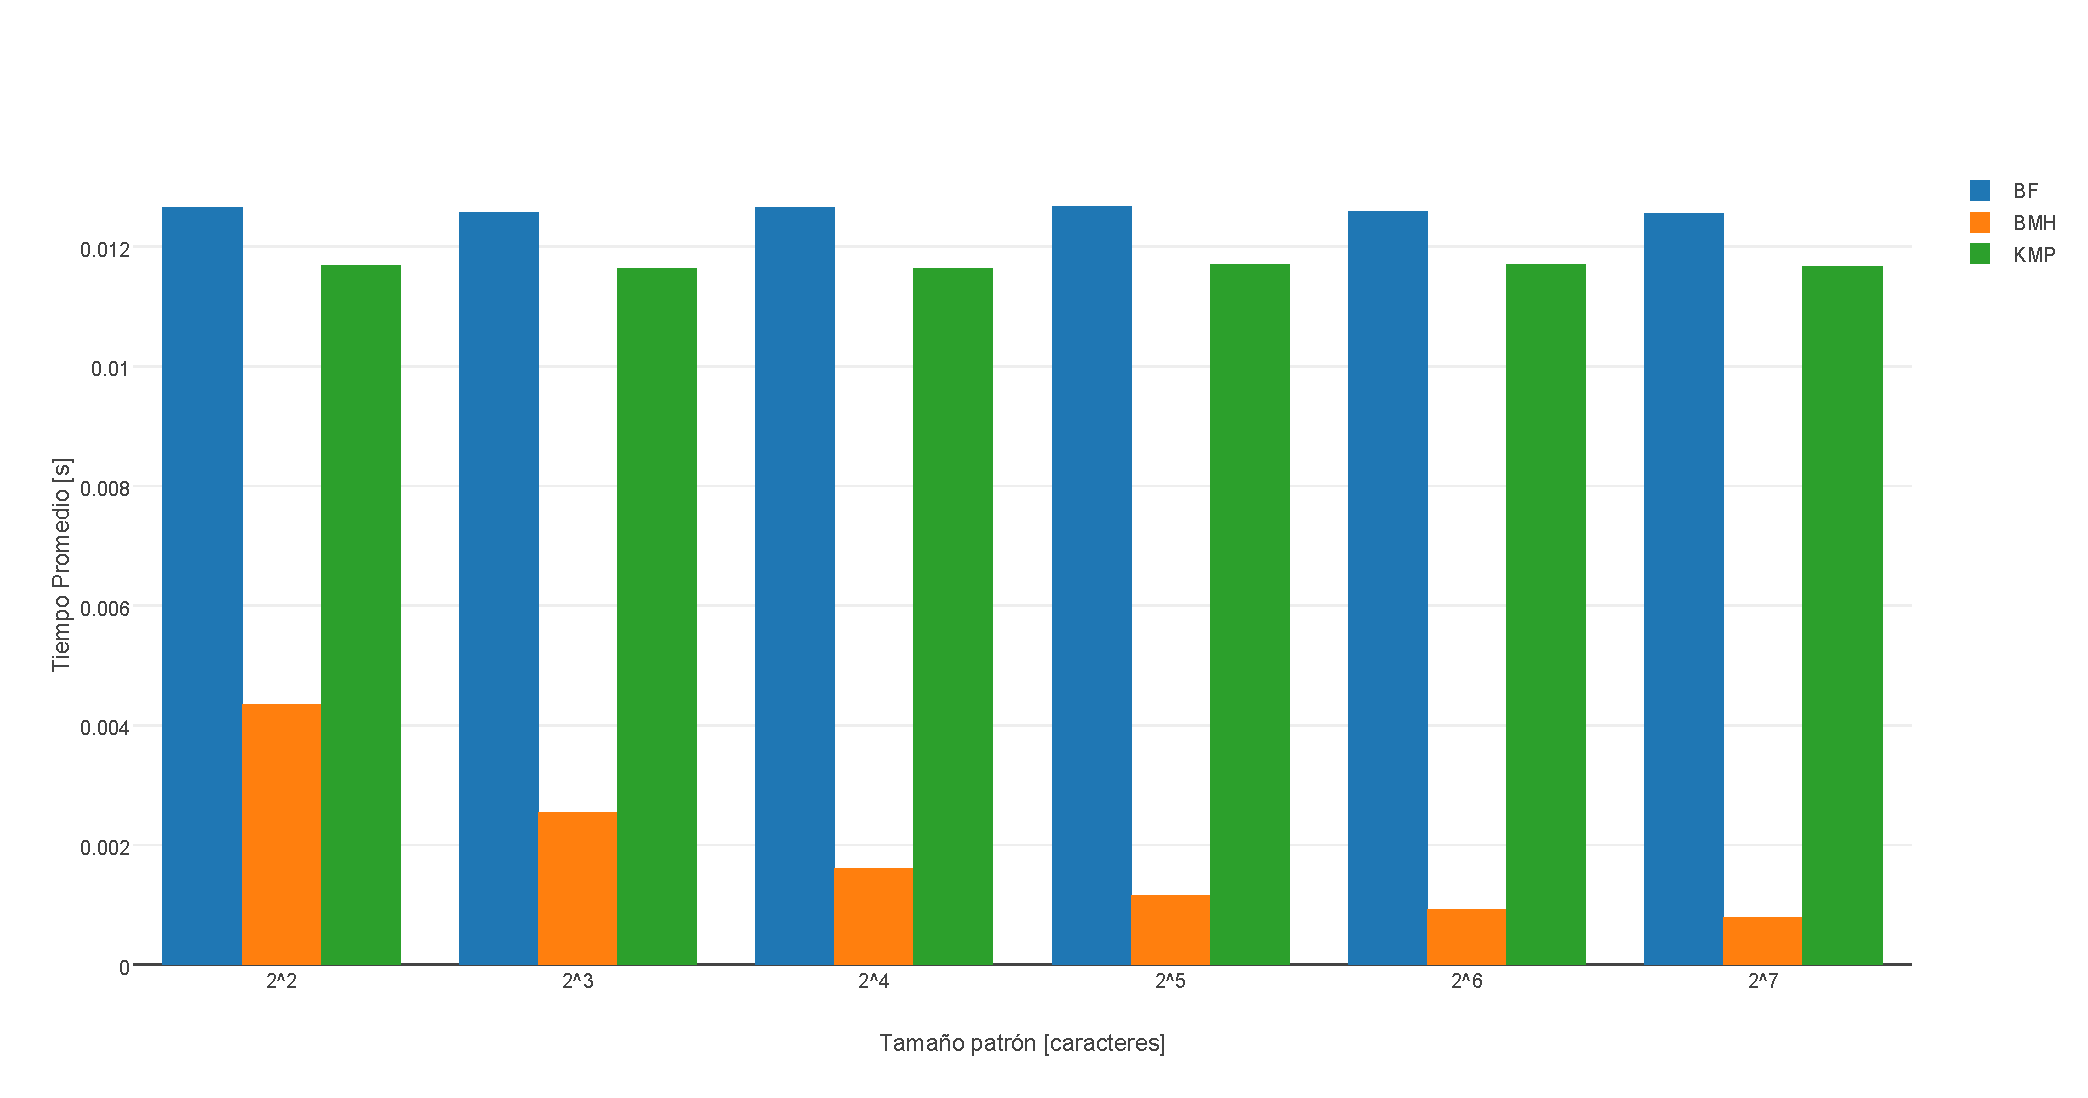
\includegraphics[scale=0.5]{img/tRLNG.pdf}
			\caption{Tiempo promedio de búsqueda para lenguaje natural} \label{construccion}
		\end{figure}
			\newpage
		\begin{figure}[ht!]
			\centering
			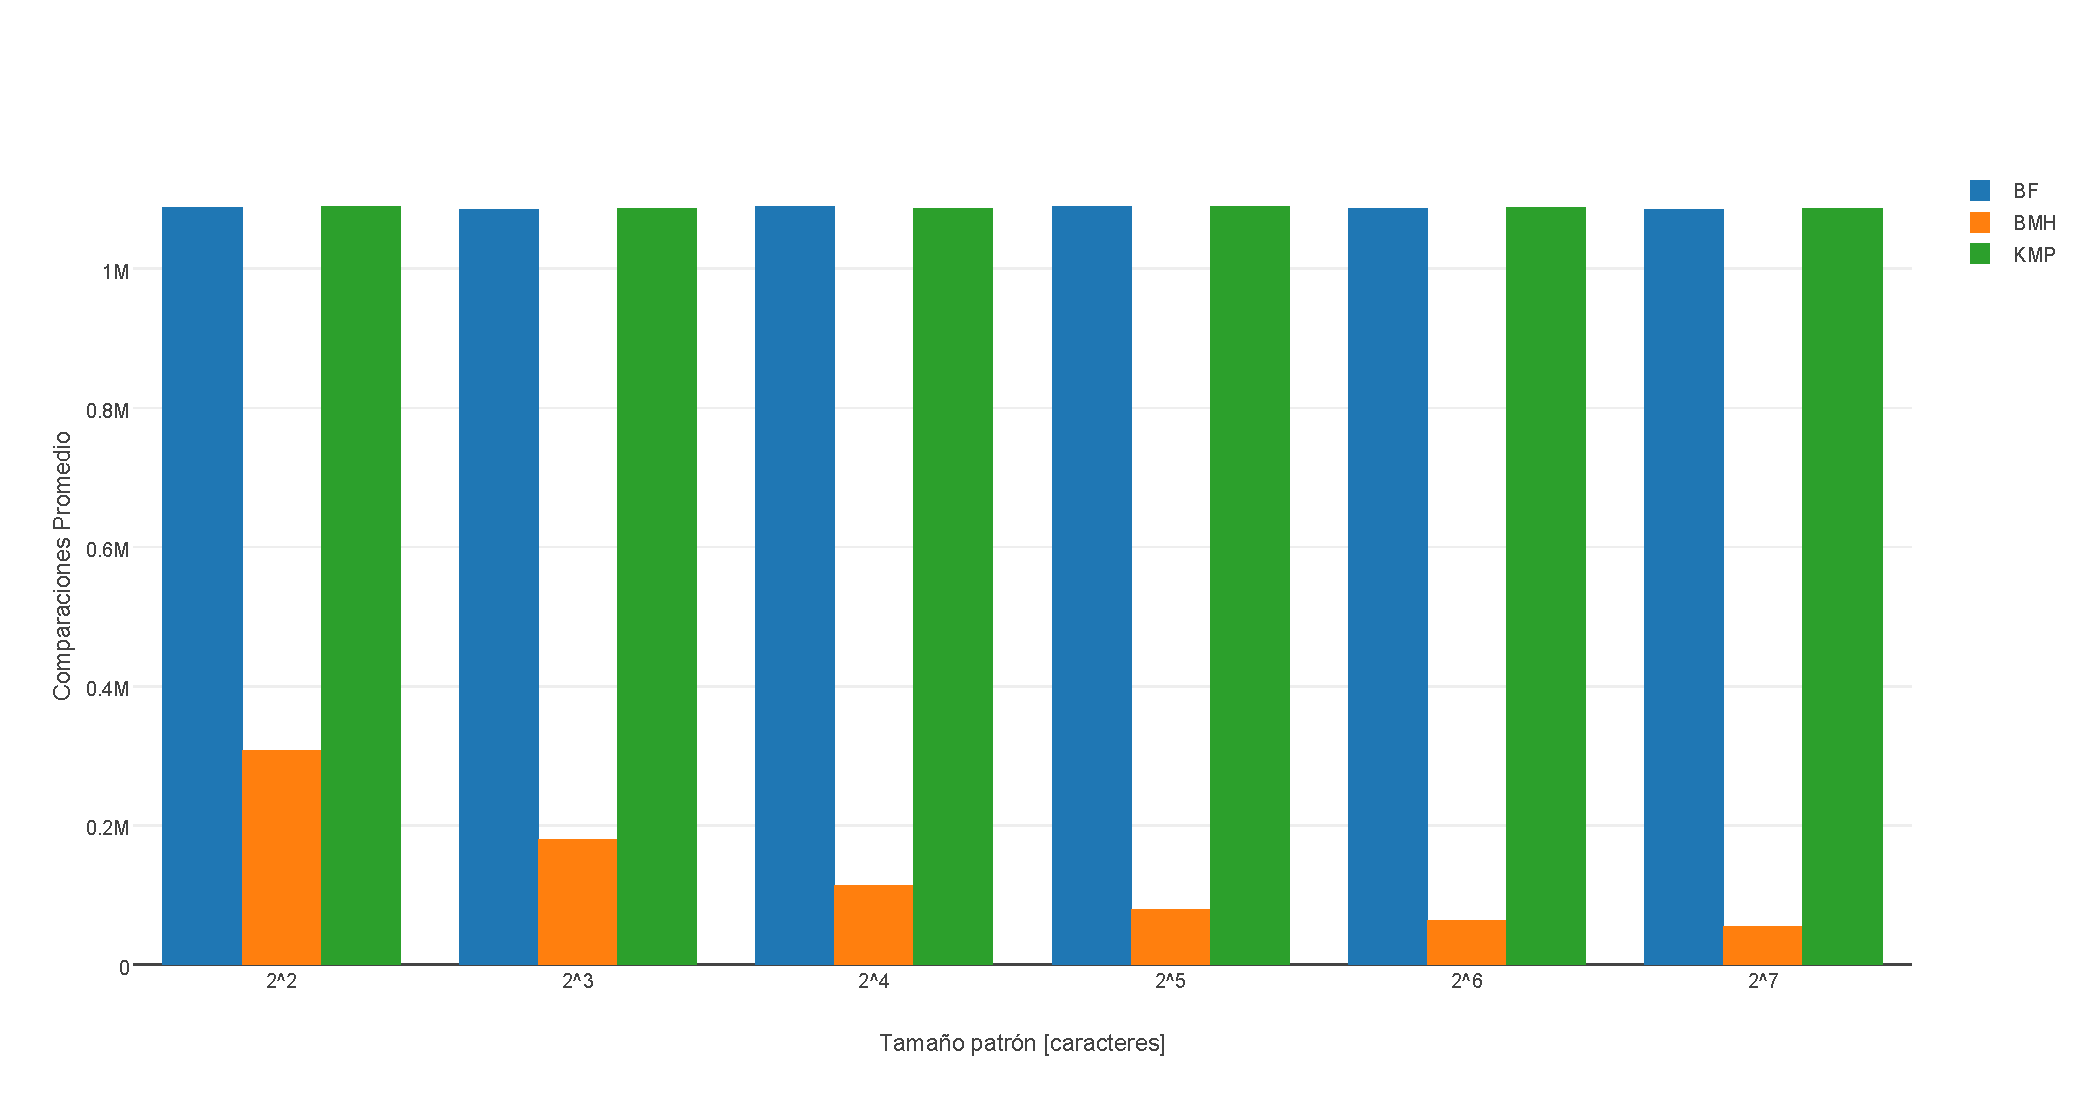
\includegraphics[scale=0.5]{img/cRLNG.pdf}
			\caption{Comparaciones promedio por búsqueda para lenguaje natural} \label{construccion}
		\end{figure}




% \begin{figure}[ht!]
% 	\centering
% 	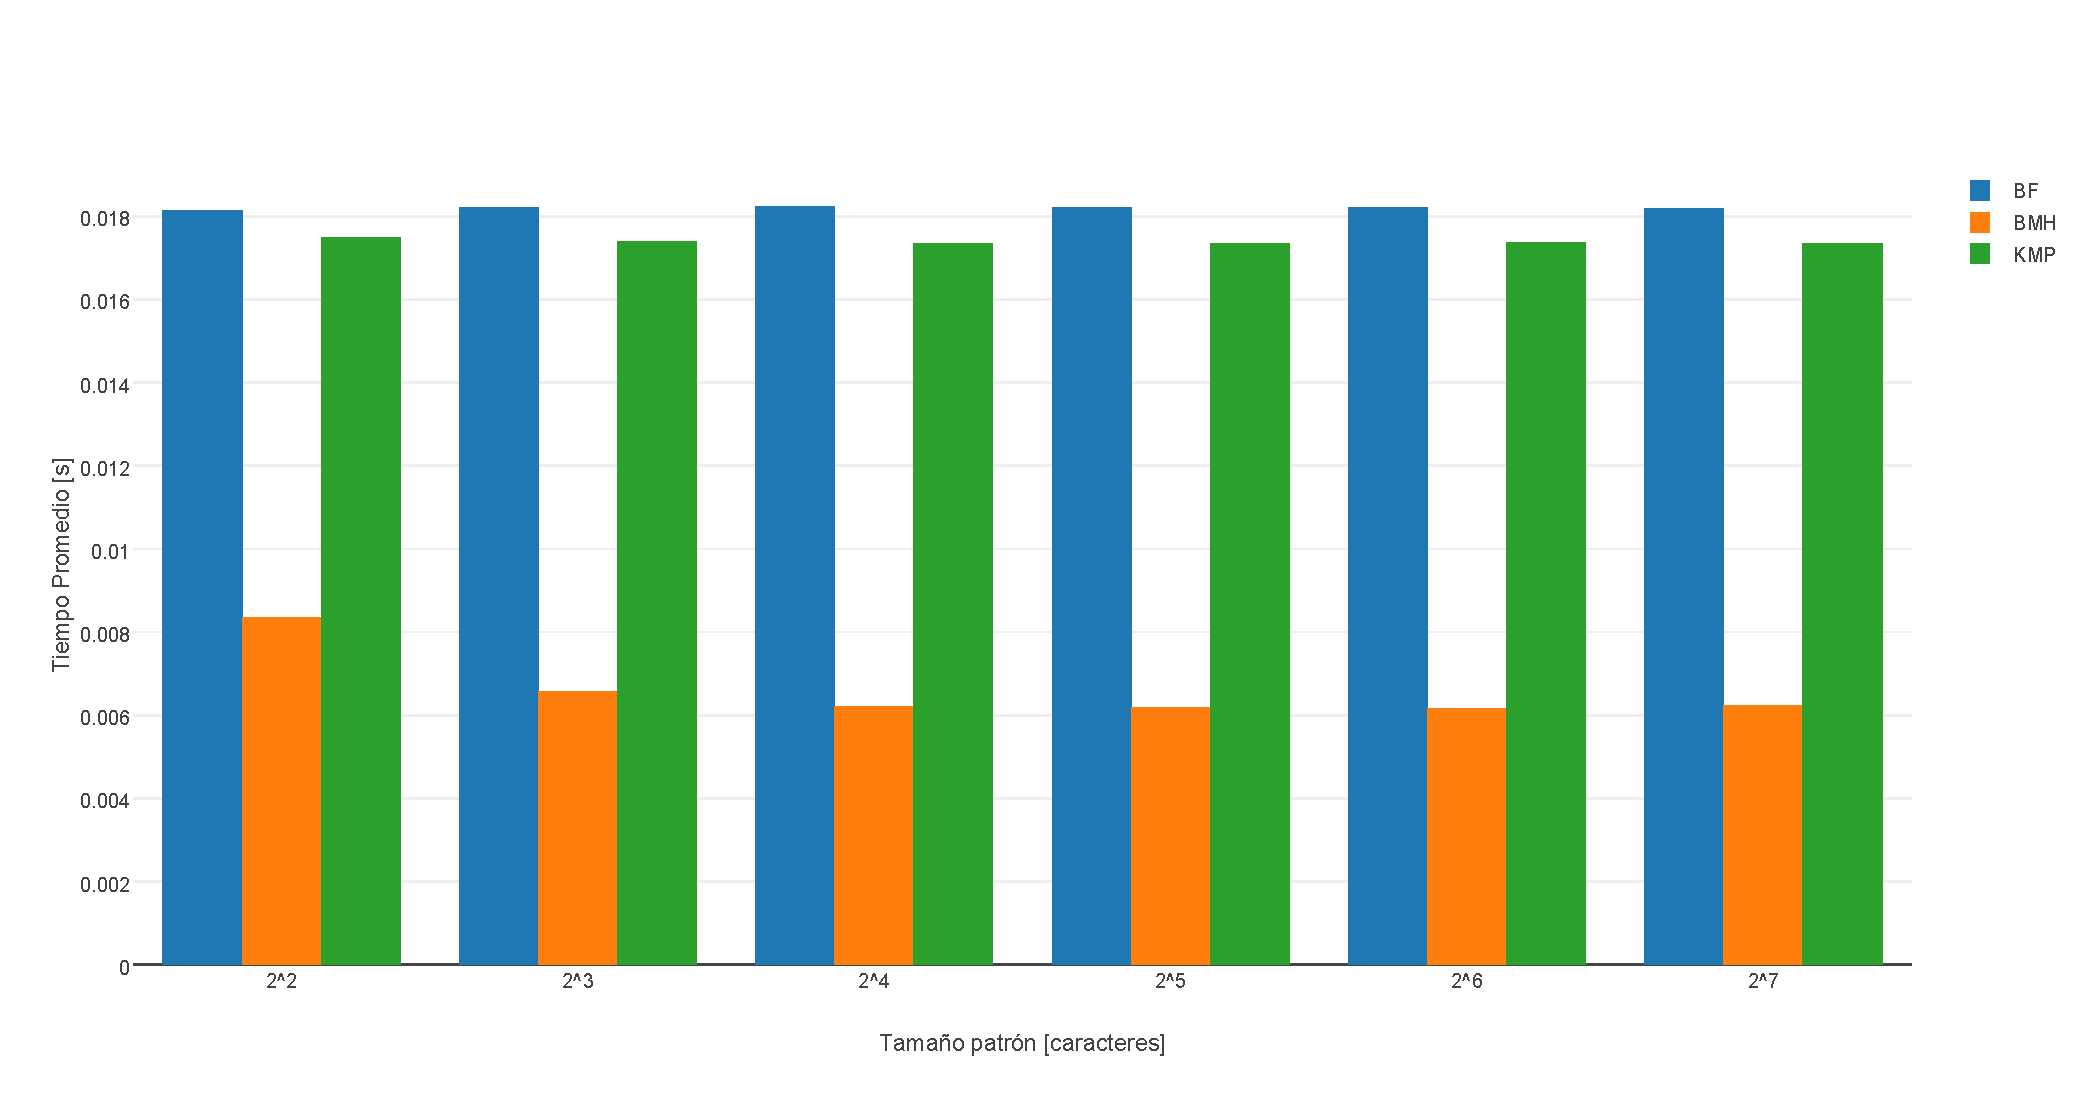
\includegraphics[scale=0.5]{img/tSDNA.pdf}
% 	\caption{Tiempo de búsqueda para cada estructura} \label{construccion}
% \end{figure}
% \begin{figure}[ht!]
% 	\centering
% 	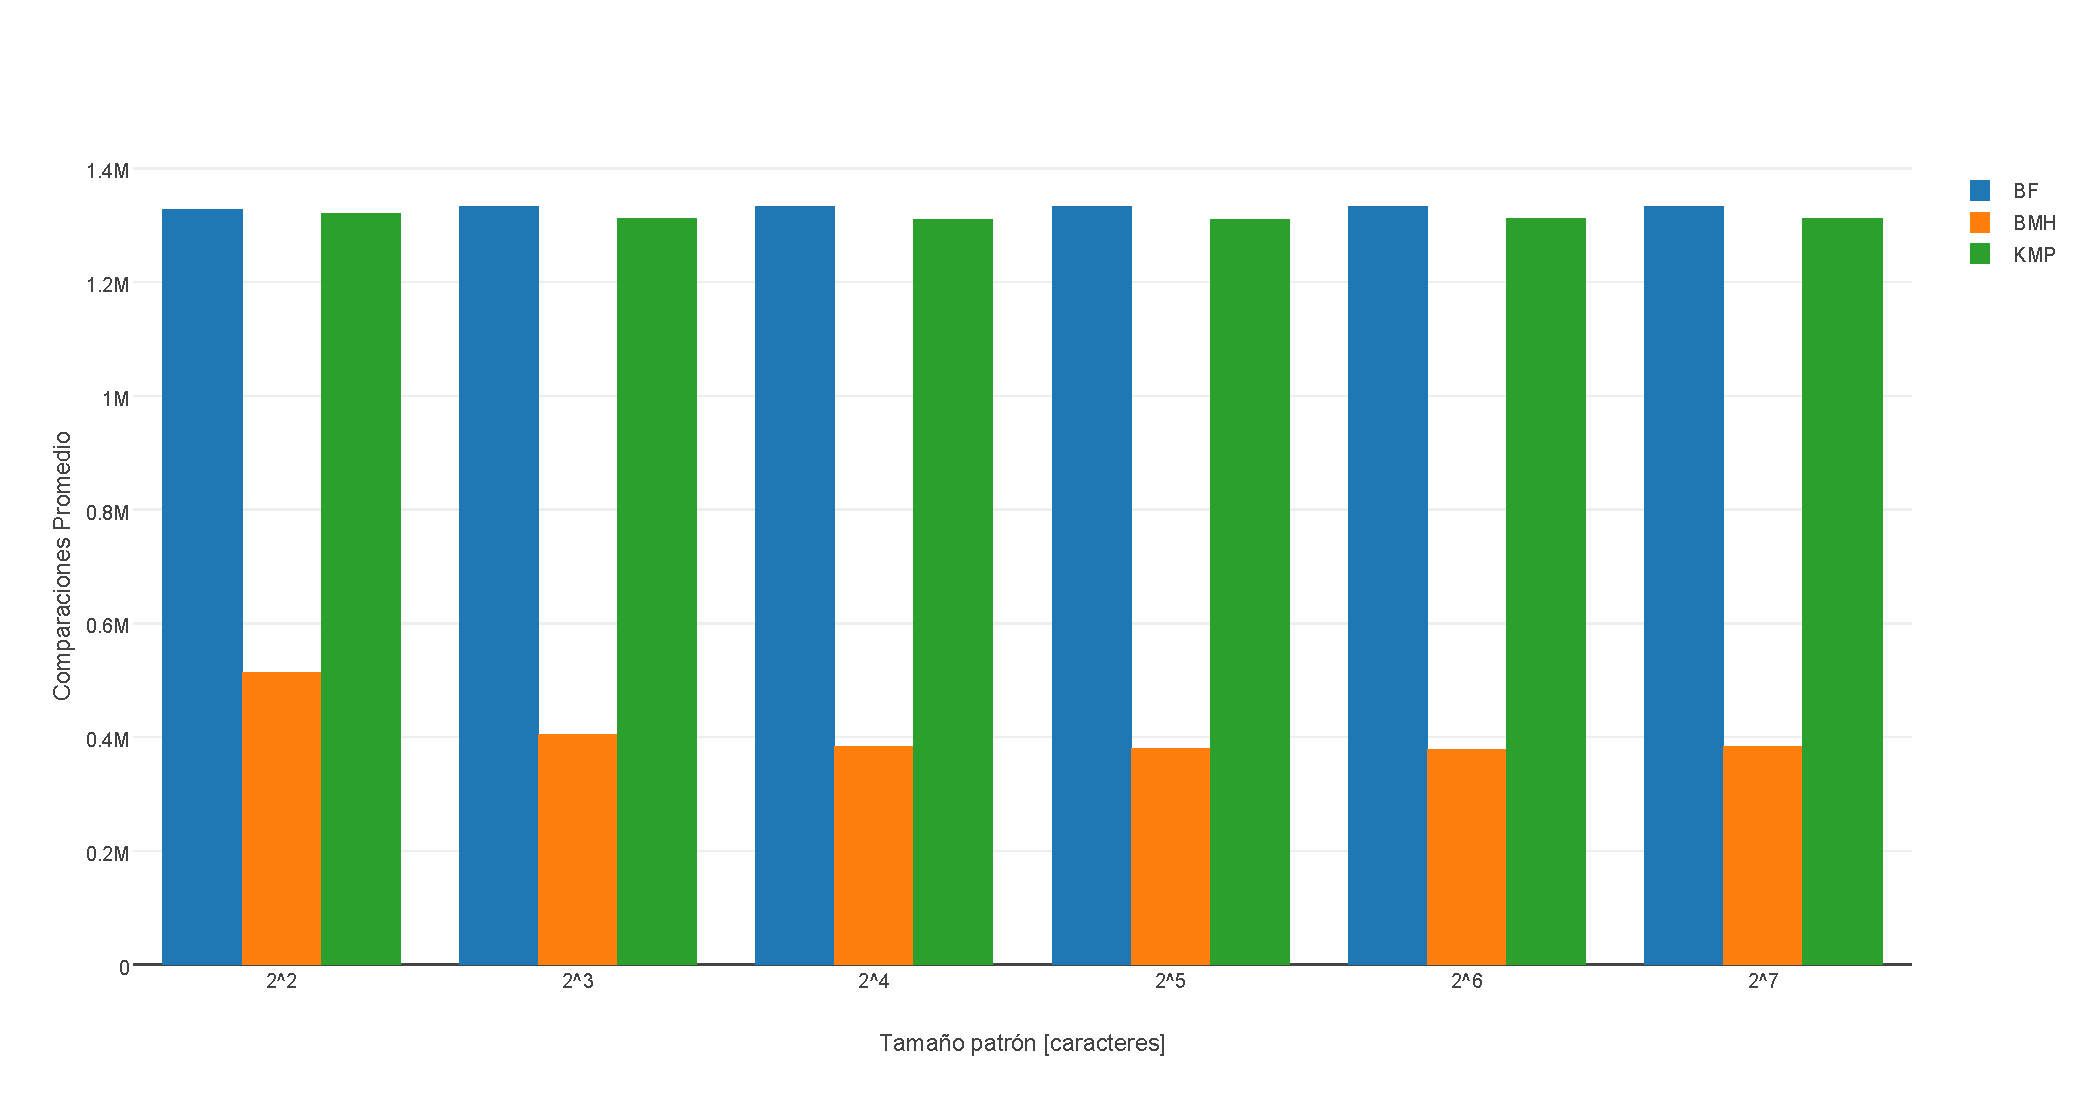
\includegraphics[scale=0.5]{img/cSDNA.pdf}
% 	\caption{Tiempo de búsqueda para cada estructura} \label{construccion}
% \end{figure}

% \begin{figure}[ht!]
% 	\centering
% 	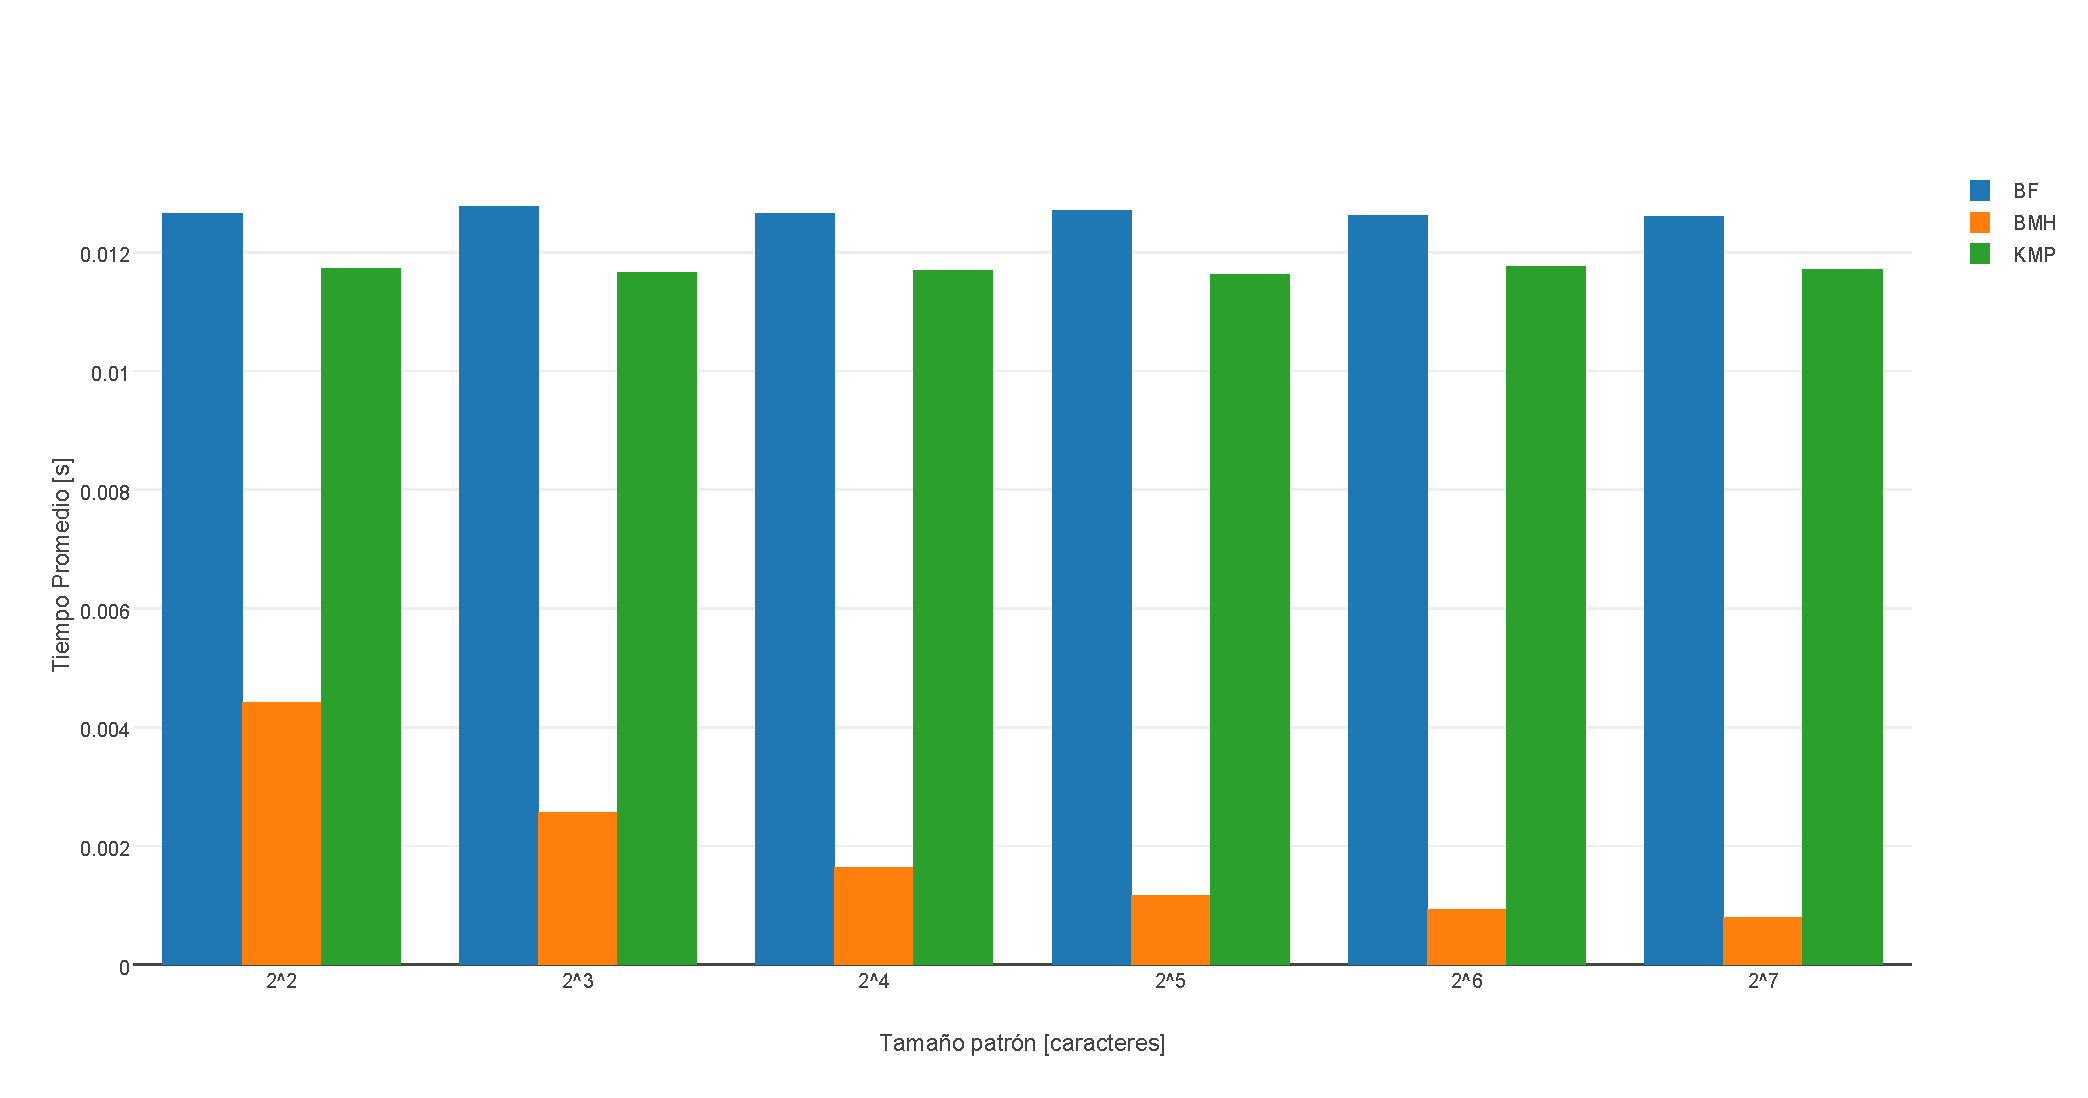
\includegraphics[scale=0.5]{img/tSLNG.pdf}
% 	\caption{Tiempo de búsqueda para cada estructura} \label{construccion}
% \end{figure}
% \begin{figure}[ht!]
% 	\centering
% 	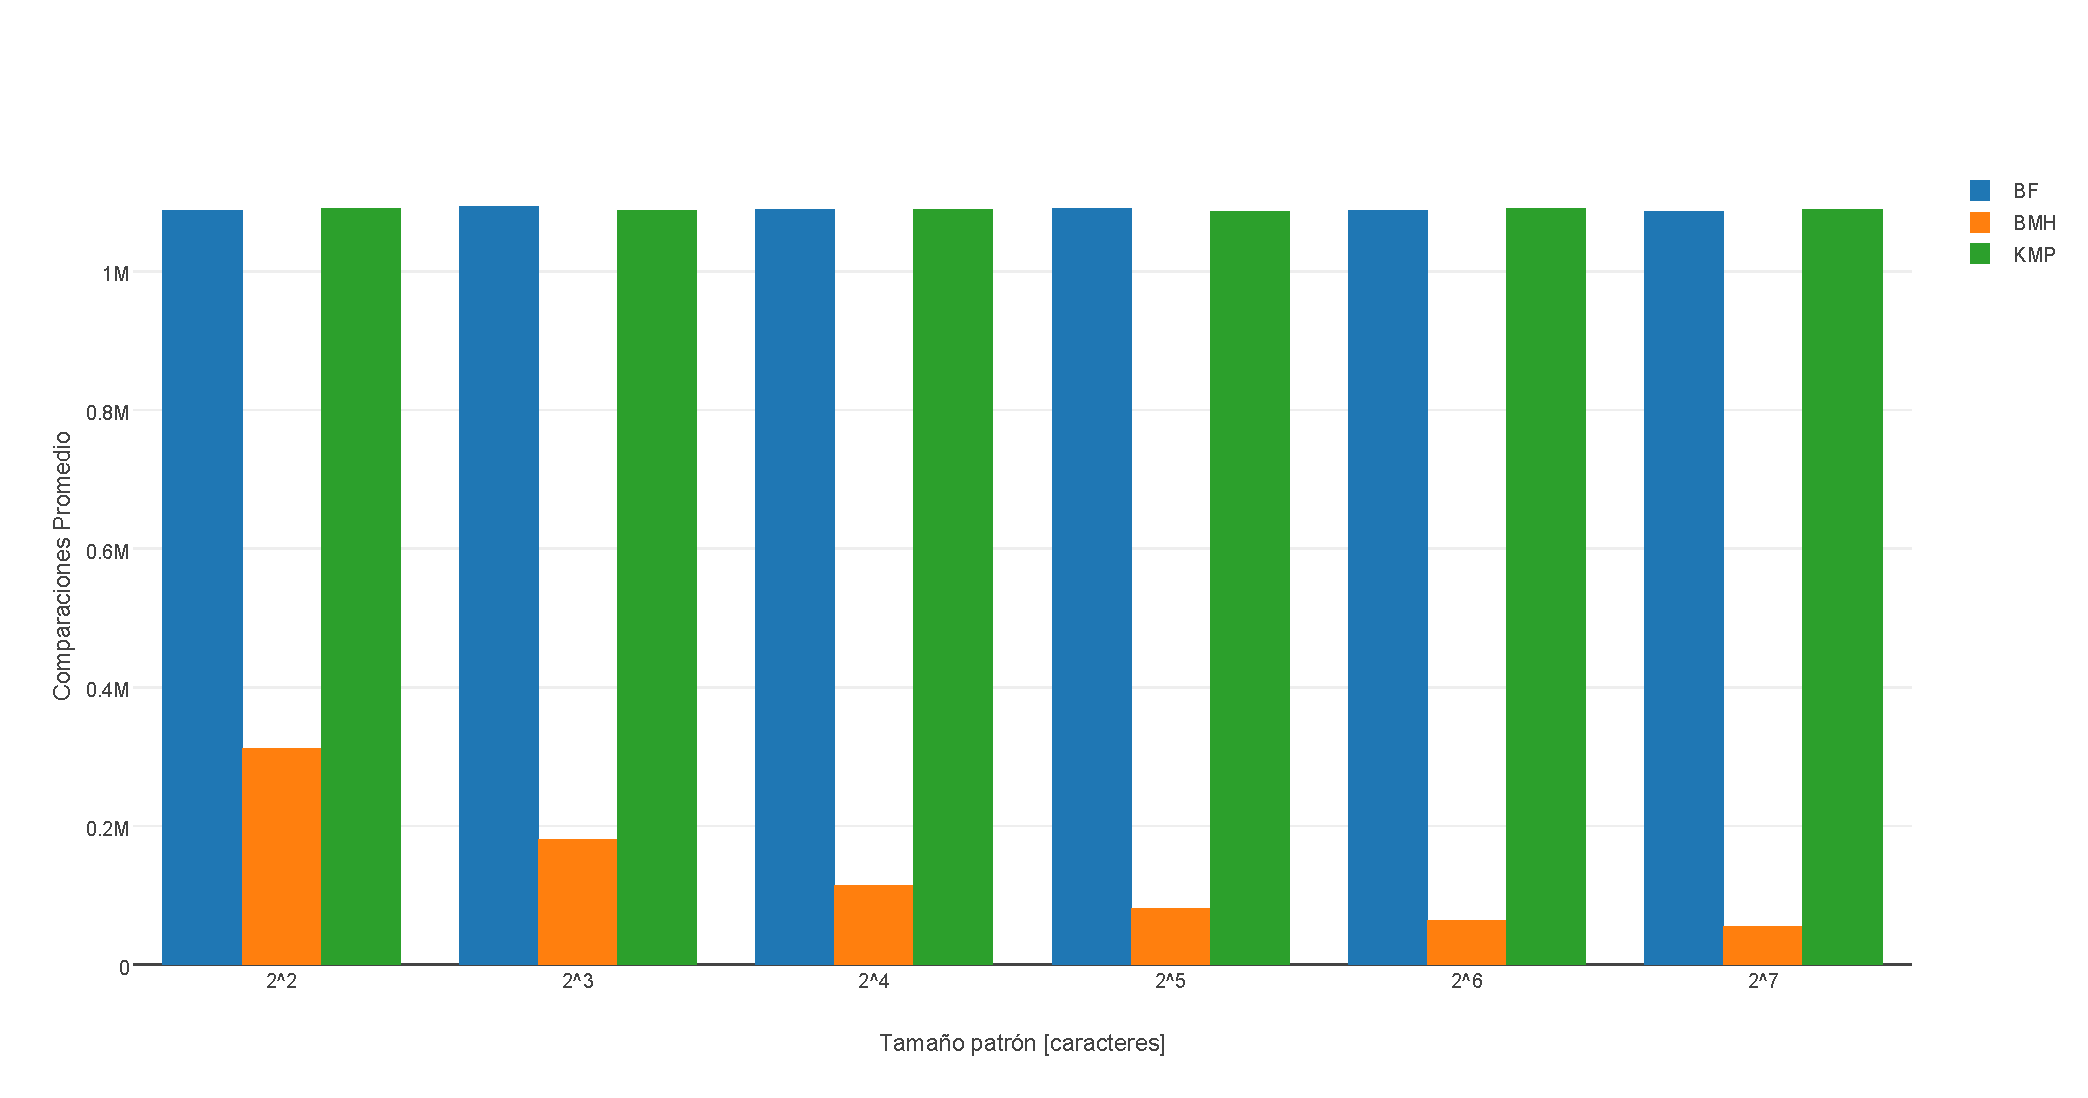
\includegraphics[scale=0.5]{img/cSLNG.pdf}
% 	\caption{Tiempo de búsqueda para cada estructura} \label{construccion}
% \end{figure}


\newpage
\section{Análisis y Conclusiones}
	En los resultados de cada algoritmo se puede confirmar como aumentar $c$ hace que mejore el rendimiento.
\subsection{Fuerza Bruta}
	No ocurre lo esperado, ya que el rendimiento no empeora al aumentar $m$.

\subsection{Knuth-Morris-Pratt}
	Este algoritmo depende de que se tengan muchas subcadenas que sean prefijo del patrón, lo que significa que va a ser mejor que
	el primer algoritmo, pero no por mucho.

\subsection{Boyer-Moore-Horspool}
	Este algoritmo se va a comportar mejor que los 2 anteriores por la forma en que salta en el texto
	al encontrar diferencias (si el caracter no se encuentra o se encuentra muy al principio se salta $m$).
	Para un $c$ pequeño, este algoritmo no va a ser tanto mejor que los anteriores, pero a medida que crezca,
	va a mejorar significativamente.

%%==================== IMAGENES =====================
%% ················ IMAGEN DOBLE ·················
%\begin{figure}[ht!] \centering
%\subfloat[Logo UChile]{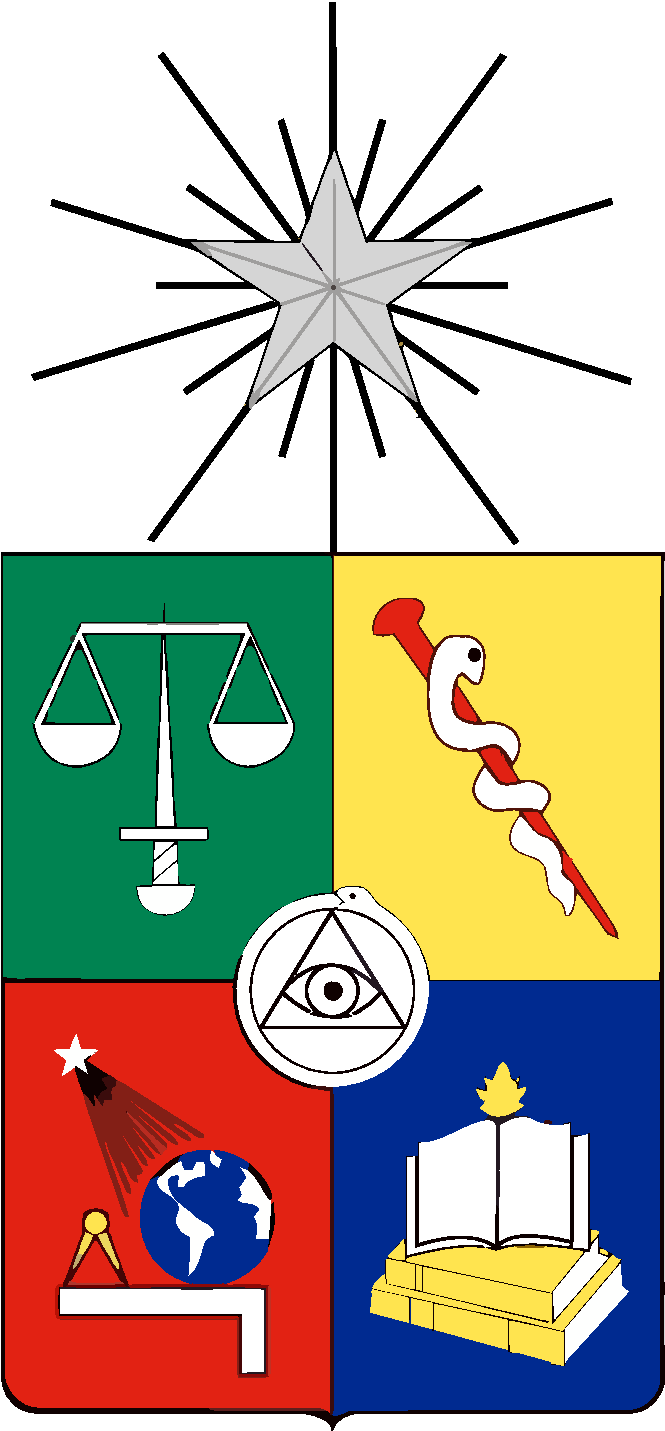
\includegraphics[scale=0.2]{img/escudoU.pdf}}
%\hspace{1cm} %Espacio horizontal
%\subfloat[Logo FCFM]{
\includegraphics[scale=0.45]{img/fcfm.png}}
%\caption{Ejemplo de imagen doble}\label{img1}
%\end{figure}
%%··········································
%
%
%A continuación la figura \ref{img2} presenta otra forma de agregar imágenes
%
%% ················ IMAGENES SIMPLES·················
%\begin{figure}[ht!]
%\centering 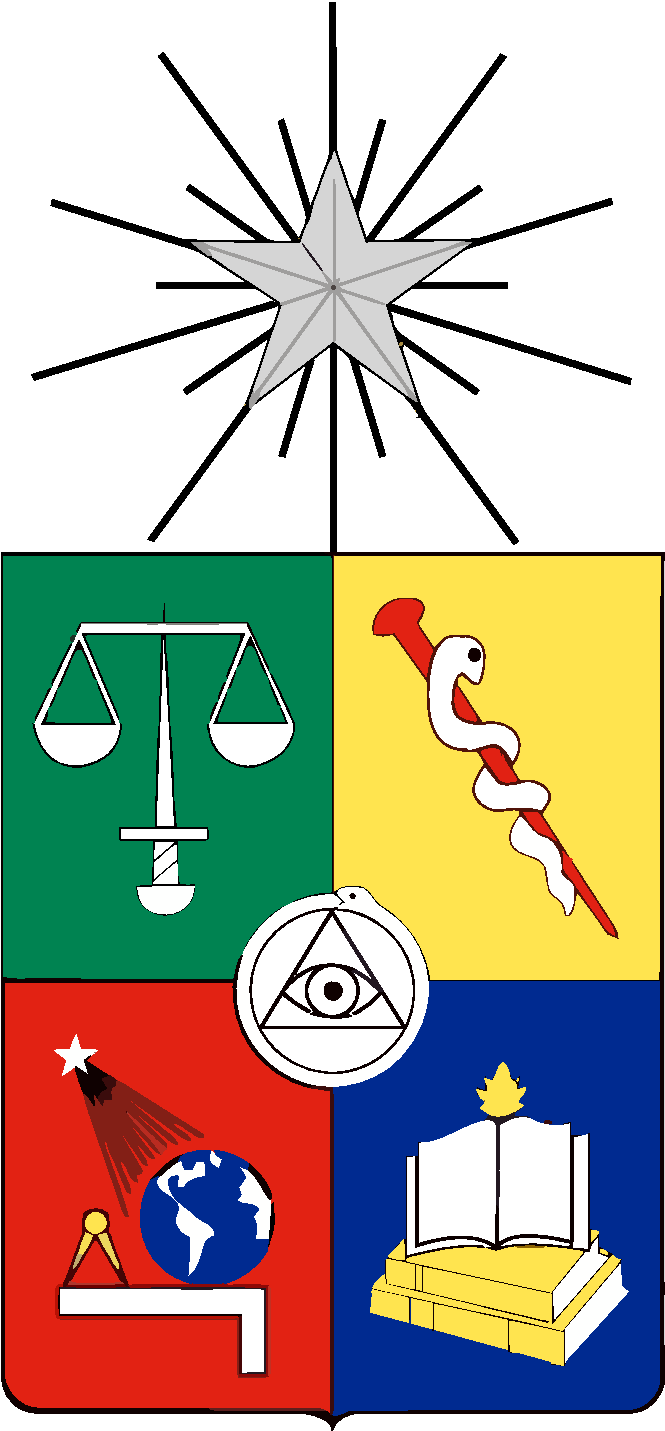
\includegraphics[scale=0.2]{img/escudoU.pdf}
%\caption{Escudo de la Universidad de Chile} \label{img2}
%\end{figure}

%%--------------------------
%
%\begin{figure}[ht!]
%\centering
%\captionsetup{justification=centering,margin=2cm}
%\includegraphics[scale=0.2]{img/fotos_alma/bunkers.JPG}
%\caption{Burros salvajes junto a los bunkers del campamento donde aloja el personal de OSF}
%\label{campamento}
%\end{figure}

%\begin{figure}[ht!]
%\centering \includegraphics[scale=0.2]{img/fotos_alma/cancha_casino.JPG}
%\caption{Multicancha y casino de OSF}
%\label{cancha}
%\end{figure}

%----------------------------
%\begin{figure}[ht!]
%\centering
%\hspace*{-2cm}
%\captionsetup{justification=centering,margin=2cm}
%\includegraphics[scale=0.3]{img/figure_2.pdf}
%\caption{Ejemplo de visualización de un perfil de temperatura usando datos de agosto de 2010}
%\label{surftemp_fig}
%\end{figure}
%\begin{figure}
%\centering
%\hspace*{-2cm}
%\captionsetup{justification=centering,margin=2cm}
%\includegraphics[scale=0.3]{img/figure_3.pdf}
%\caption{Ejemplo de visualización de un perfil de temperatura usando datos de agosto de 2010}
%\label{intliq_fig}
%\end{figure}
%%··········································



%%============== TABLAS ===============
%\begin{table}[h]
% \centering
% \caption{Headers, identificadores y descripción}
% \begin{tabular}{|| c | c | p{7	cm}||}
% \hline
% Identificador de header & Tipo de medición & Descripción \\ [0.5ex]
% \hline\hline
% 10 & - & No se usa (tampoco se describe en el manual)\\
% \hline
% 80 & - & No se usa (tampoco se describe en el manual) \\
% \hline
% 100 & 101 & Tipo de medición y título de los 4 tipos de perfiles\\
% \hline
% 200 & 201 & Header para mediciones meteorológicas a nivel de superficie\\
% \hline
% 300 & 301 & Header para mediciones escalares e integradas\\
% \hline
% 400 & 401, 402, 403, 404 & Ángulo de observación y arreglo de valores de 			altura, la varible independientele (58 valores, de 0 a 10 km), para todos 		los perfiles.\\
% \hline
% \end{tabular}
%\end{table}
%\newpage
%
%Las siguientes cuatro filas contienen el tipo de medición ``101", y especifican el tipo de medición para los cuatro tipos de perfiles.
%
%\begin{table}[h]
% \centering
% \caption{Tipo de perfil y datos}
% \begin{tabular}{||c|c|c|c|c||}
% \hline
% N° de medición & Fecha/Tiempo & 100 &	Tipo de medición & Título \\ [0.5ex]
% \hline\hline
% 1	& 10/07/14 22:07:14 & 101 & 401 & Temperature(K) \\
% \hline
% 2	& 10/07/14 22:07:14 & 101 & 402 & Vapor Density $(g/m^3)$ \\
% \hline
% 3	& 10/07/14 22:07:14 & 101 & 403 & Liquid Density $(g/m^3)$ \\
% \hline
% 4	& 10/07/14 22:07:14 & 101 & 404 & Relative Humidity (\%) \\
% \hline
% \end{tabular}
%\end{table}
%
%El resto de las filas son mediciones (de tipo 201, 301, 401, 402, 403 y 404). \textbf{Estas son las medidas que van a hacer almacenadas en la base de datos}
%\begin{table}[h]
% \centering
% \caption{Ejemplo de mediciones meteorológicas a nivel de superficie y su correspondiente header}
% \begin{tabular}{||c|c|c|c|c|c|c|c||}
% \hline
% Record & Date/Time & 200 & Tamb(K) & Rh(\%) & Pres(mb) & Tir(K) & Rain \\ [0.5ex]
% \hline\hline
% 25 & 10/07/14 22:08:13 & 201 & 276.032 & 10.13 & 557.48 & 191.09 & 0 \\
% \hline
% \end{tabular}
%\end{table}
%
%\newpage
%\begin{table}[h]
% \centering
% \caption{Ejemplo de mediciones de valores scalares e integrados y su correspondiente header}
% \begin{tabular}{||c|c|c|c|c|c|c||}
% \hline
% Record & Date/Time & 300 &	Int. Vapor(cm) & Int. Liquid(mm) & Cloud Base(km) \\ [0.5ex]
% \hline\hline
% 42	& 10/07/14 22:08:56 & 301 & 0.077 & 0 & -1 \\
% \hline
% \end{tabular}
%\end{table}
%
%\begin{table}[h]
% \centering
% \caption{Ejemplo de perfiles y sus correspondientes headers}
% \begin{tabular}{||c|c|c|c|c|c|c||}
% \hline
% Record & Date/Time & 400 &	LV2 Processor(angle) & 0 & ... & 10 \\ [0.5ex]
% \hline\hline
% 46 & 10/07/14 22:09:41 & 401 &	Zenith & 276.017 & ... & 259.11 \\
% \hline
% 53	& 10/07/14 22:09:43 & 402 &	Angle Scan(N) &	0.623 & ... & 0.007 \\
% \hline
% 57	& 10/07/14 22:09:43 & 403 &	Angle Scan(S) &	0.021 & ... & 0.005 \\
% \hline
% 61	& 10/07/14 22:09:43 & 404 &	Angle Scan(A) &	2.805 & ... & 0.336 \\
% \hline
% \end{tabular}
%\end{table}


% ============= REFERENCIAS ==============
%\newpage
%
%\section{Referencias}
%\begin{thebibliography}{99}
%	\bibitem{nodoPag} R. Jacob Baker, \textit{CMOS. Circuit Design, Layout, and Simulation}, 2nd ed., USA: IEEE Press, 2005
%	\bibitem{Bojan} asdasdas
%
%\end{thebibliography}


% ============= FIN DE DOCUMENTO ==============
\end{document}
